\documentclass[10pt,letterpaper]{article}
\usepackage[utf8]{inputenc}
\usepackage[T1]{fontenc}
\usepackage{lmodern}
\usepackage{environ}
\usepackage{color}
\usepackage{amsmath,amsthm,amsfonts,amssymb}
\usepackage{verbatim}
\usepackage{graphicx}
\usepackage{subfigure}
\usepackage{multirow}
\usepackage[capitalise]{cleveref}
%%%%%%%%%%%%%%%%%%%%%%%%%%%%%%%%%%%%%%%%%%%%%
%%%%%%%%%%%%%%%%%%%%%%%%%%%%%%%%%%%%%%%%%%%%%
%%%%%%%%%%%%%%%%%%%%%%%%%%%%%%%%%%%%%%%%%%%%%

\newcommand{\X}{\ensuremath{\mathcal{X}}}
\newcommand{\R}{\ensuremath{\mathcal{R}}}
\newcommand{\mP}{\ensuremath{\mathcal{P}}}
\newcommand{\mM}{\ensuremath{\mathcal{M}}}
\newcommand{\ip}[2]{\ensuremath{\langle #1, #2 \rangle}}
\newcommand{\grad}{\nabla}
\newcommand{\one}{\ensuremath{\mathbf{1}}}
\newcommand{\co}{\mbox{co}}

\newcommand{\calL}{{\mathcal{L}}}
\newcommand{\rank}{{\calL(A)}}
\newcommand{\calO}{{\mathcal{O}}}
\newcommand{\calP}{{\mathcal{P}}}

\newcommand{\uni}{{\rank^n}}
\newcommand{\sca}{{\scr^{\alpha}}}
\newcommand{\sort}{\text{SORT}}
\newcommand{\phia}{\phi^{\alpha}}
\newcommand{\mmphia}{\mm^{\phia}}

\newcommand{\muhat}{\hat{\mu}}
\newcommand{\that}{\hat{\theta}}

\DeclareMathOperator*{\argmax}{arg\,max}
\DeclareMathOperator*{\argmin}{arg\,min}
\newcommand{\eps}{\epsilon}

\newtheorem{theorem}{Theorem}
\newtheorem{lemma}{Lemma}
\newtheorem{conjecture}{Conjecture}
\newtheorem{claim}{Claim}
\newtheorem{proposition}{Proposition}
\newtheorem{corollary}{Corollary}

\newenvironment{definition}[1][Definition]{\begin{trivlist}
\item[\hskip \labelsep {\bfseries #1}]}{\end{trivlist}}
\newenvironment{example}[1][Example]{\begin{trivlist}
\item[\hskip \labelsep {\bfseries #1}]}{\end{trivlist}}
\newenvironment{remark}[1][Remark]{\begin{trivlist}
\item[\hskip \labelsep {\bfseries #1}]}{\end{trivlist}}


\newcount\Comments
\Comments=1
\newcommand{\kibitz}[2]{\ifnum\Comments=1\textcolor{#1}{#2}\fi}
\newcommand{\csl}[1]{\kibitz{blue} {[SL: #1]}}
\newcommand{\cns}[1]{\kibitz{red} {[NS: #1]}}

\newcommand{\nt}{NT}

%%%%%%%%%%%%%%%%%%%%%%%%%%%%%%%%%%%%%%%%%%%%%
%%%%%%%%%%%%%%%%%%%%%%%%%%%%%%%%%%%%%%%%%%%%%
%%%%%%%%%%%%%%%%%%%%%%%%%%%%%%%%%%%%%%%%%%%%%

\title{Euclidean Voting}
\author{S\'{e}bastien Lahaie\\Microsoft Research New York, USA\\slahaie@microsoft.com \and Nisarg Shah\\Carnegie Mellon University, USA\\nkshah@cs.cmu.edu}
\date{}
\begin{document}
\maketitle

%%%%%%%%%%%%%%%%%%%%%%%%%%%%%%%%%%%%%%%%%%%%%
%%%%%%%%%%%%%%%%%%%%%%%%%%%%%%%%%%%%%%%%%%%%%
%%%%%%%%%%%%%%%%%%%%%%%%%%%%%%%%%%%%%%%%%%%%%

\section{Preliminaries}

Let $A$ denote the set of $m$ alternatives, and $\rank$ and $\calO$ denote the space of rankings of alternatives and outcomes, respectively. Thus, $|\rank| = m!$, and let $k = |\calO|$. A profile $\pi \in \rank^n$ is a collection of votes (rankings). For any profile $\pi$, let $n(\pi,\sigma)$ denote the number of times $\sigma$ appears in $\pi$. Let $\sigma_1,\ldots,\sigma_{m!}$ denote a fixed reference order of the rankings in $\rank$. 

For any two profiles $\pi_1$ and $\pi_2$, let $\pi_1+\pi_2$ be the union profile such that $n(\pi_1+\pi_2,\sigma) = n(\pi_1,\sigma)+n(\pi_2,\sigma)$ for every $\sigma \in \rank$. Similarly, for any profile $\pi$, let $c \pi$ be the profile such that $n(c \pi,\sigma) = c \cdot n(\pi,\sigma)$ for every $\sigma \in \rank$. 

%%%%%%%%%%%%%%%%%%%%%%%%%%%%%%%%%%%%%%%%%%%%%

\begin{definition}[Voting Rule]
A \emph{voting rule} (more technically, a social welfare function - SWF) $r : \rank^n \rightarrow \calP(\rank)\setminus\{\emptyset\}$ is a function that maps every profile of votes to a set of tied rankings. 
\end{definition}

Note that a voting rule can never output an empty set.

%%%%%%%%%%%%%%%%%%%%%%%%%%%%%%%%%%%%%%%%%%%%%

\begin{definition}[Anonymity]
A voting rule $r$ is called \emph{anonymous} if it only depends on the number of times each ranking appears in the profile: for every profiles $\pi_1$ and $\pi_2$ such that $n(\pi_1,\sigma) = n(\pi_2,\sigma)$ for every $\sigma \in \rank$, $r(\pi_1) = r(\pi_2)$. 
\end{definition}

%%%%%%%%%%%%%%%%%%%%%%%%%%%%%%%%%%%%%%%%%%%%%

\begin{definition}[Rank-Distinguishability]
A voting rule $r$ is called \emph{rank-distinguishing} if it can distinguish between any two rankings: for every two rankings $\sigma, \sigma' \in \rank$ ($\sigma \neq \sigma'$), there exists a profile $\pi$ such that exactly one of $\sigma$ or $\sigma'$ is in $r(\pi)$. 
\end{definition}

In this paper, we only consider rank-distinguishing voting rules.

%%%%%%%%%%%%%%%%%%%%%%%%%%%%%%%%%%%%%%%%%%%%%

\begin{definition}[Unanimity]
A voting rule $r$ is said to satisfy \emph{unanimity} if on every profile that consists of copies of a single ranking, it uniquely outputs that ranking: for every profile $\pi$ such that $n(\pi,\sigma) > 0$ for some $\sigma \in \rank$ and $n(\pi,\sigma') = 0$ for all $\sigma' \neq \sigma$, $r(\pi) = \{\sigma\}$. 
\end{definition}

%%%%%%%%%%%%%%%%%%%%%%%%%%%%%%%%%%%%%%%%%%%%%
\begin{definition}[Neutrality]
Given any profile $\pi = (\sigma_1,\ldots,\sigma_n)$, let $\tau \pi = (\tau \sigma_1,\ldots,\tau \sigma_n)$ be the profile where each vote is permuted according to $\tau$. Similarly, given any set of rankings $S$, let $\tau S = \{\tau \sigma | \sigma \in S\}$. A voting rule $r$ is called \emph{neutral} if for every profile $\pi$ and permutation $\tau$, we have $r(\tau \pi) = \tau r(\pi)$. 
\end{definition}

%%%%%%%%%%%%%%%%%%%%%%%%%%%%%%%%%%%%%%%%%%%%%

\begin{definition}[Consistency] %and Weak Consistency]
A social welfare function $r$ is called \emph{consistent} (for rankings) if for every profiles $\pi_1$ and $\pi_2$ such that $r(\pi_1) \cap r(\pi_2) \neq \emptyset$, $r(\pi_1+\pi_2) = r(\pi_1) \cap r(\pi_2)$. %A social welfare function $r$ is called weakly consistent (for rankings) if for every profiles $\pi_1$ and $\pi_2$ such that $r(\pi_1) = r(\pi_2)$, we have $r(\pi_1+\pi_2) = r(\pi_1) = r(\pi_2)$. 
\end{definition}

%%%%%%%%%%%%%%%%%%%%%%%%%%%%%%%%%%%%%%%%%%%%%

\begin{definition}[Connectedness]
A voting rule $r$ is called \emph{connected} if for any two profiles $\pi_1$ and $\pi_2$ with $r(\pi_1) \cap r(\pi_2) \neq \emptyset$, there exist non-negative integers $c$ and $d$ such that $r(\pi_1) \cap r(c \pi_1 + d \pi_2) \neq \emptyset$ and $r(\pi_1) \neq r(c \pi_1 + d \pi_2)$. 
\end{definition}

%%%%%%%%%%%%%%%%%%%%%%%%%%%%%%%%%%%%%%%%%%%%%

\cns{Check if this is equivalent/related to continuity defined by Conitzer et al.~\cite{CRX09}. Then we can add that to Proposition~\ref{prop:properties}.}
\begin{definition}[Continuity]
Two profiles $\pi_1$ and $\pi_2$ satisfy $\pi_1 \approx \pi_2$ if they differ by one vote: for some $\sigma$ and $\sigma'$, $n(\pi_1,\sigma) = n(\pi_2,\sigma)-1$, $n(\pi_1,\sigma') = n(\pi_2,\sigma')+1$, and for every $\sigma \in \rank\setminus\{\sigma,\sigma'\}$, $n(\pi_1,\sigma) = n(\pi_2,\sigma)$. A voting rule $r$ is called \emph{continuous} if for every profile $\pi$ and ranking $\sigma$, $\sigma \notin r(\pi)$ implies that there exists integer $k$ such that for every profile $\pi' \approx k \pi$, $\sigma \notin r(\pi')$. 
\end{definition}

%%%%%%%%%%%%%%%%%%%%%%%%%%%%%%%%%%%%%%%%%%%%%
%%%%%%%%%%%%%%%%%%%%%%%%%%%%%%%%%%%%%%%%%%%%%
%%%%%%%%%%%%%%%%%%%%%%%%%%%%%%%%%%%%%%%%%%%%%

\section{Background on Mean Proximity Rules and Generalized Scoring Rules}

%%%%%%%%%%%%%%%%%%%%%%%%%%%%%%%%%%%%%%%%%%%%%

\begin{definition}[Mean Proximity Rules (Zwicker~\cite{Zwicker08a})]
A voting rule is called a \emph{mean proximity rule} if there exists an input embedding $\phi : \rank \rightarrow \mathbb{R}^k$ and an output embedding $\psi: \calO \rightarrow \mathbb{R}^k$ such that for any profile $\pi$ with $n$ votes, $r(\pi) = \argmin_{o \in \calO} \|\psi(o) - mean(\pi) \|$, where $mean(\pi) = (1/n) \cdot \sum_{\sigma \in \rank} n(\pi,\sigma) \cdot \phi(\sigma)$ is the mean of the input embeddings of the votes in $\pi$ (along with multiplicity). 
\end{definition}

%%%%%%%%%%%%%%%%%%%%%%%%%%%%%%%%%%%%%%%%%%%%%

\begin{definition}[Generalized Scoring Rules (Zwicker~\cite{Zwicker08a})]
A voting rule is called a \emph{generalized scoring rule} if there exists a scoring function $s : \rank \times \calO \rightarrow \mathbb{R}$ such that for any profile $\pi$, $r(\pi) = \argmax_{o \in \calO} \sum_{\sigma \in \rank} n(\pi,\sigma) \cdot s(\sigma,o)$. 
\end{definition}

%%%%%%%%%%%%%%%%%%%%%%%%%%%%%%%%%%%%%%%%%%%%%

%\begin{proposition}[Corollary~4.2.3, Zwicker~\cite{Zwicker08a}]
%Let $A = \{u_1,\ldots,u_l\}$ be a set of $l$ vectors in $\mathbb{R}^k$. Let $B = \{v_1,\ldots,v_p\}$ be a set of $p$ vectors in $\mathbb{R}^k$. Then, the discrete mean in $A$ of vectors in $B$ is the vector in $A$ that is closest to the Euclidean mean of vectors in $B$. That is,
%$$
%\argmin_{u_i \in A} \sum_{v_j \in B} \|u_i - v_j\|^2 = \argmin_{u_i \in A} \|u_i - (1/p) \cdot \sum_{v_j \in B} v_j\|.
%$$
%\label{prop:discrete-mean}
%\end{proposition}

For these two classes of voting rules, we have an elegant equivalence theorem by Zwicker~\cite{Zwicker08a}. The theorem uses an important result shown below.

\begin{proposition}[Zwicker~\cite{Zwicker08a}]
For any embeddings $\phi,\psi : \rank \rightarrow \mathbb{R}^k$ and any profile $\pi$,
$$
\argmin_{o \in \calO} \|\psi(o)-mean(\pi)\| = \argmin_{o \in \calO} \sum_{\sigma \in \rank} n(\pi,\sigma) \cdot \|\psi(o)-\phi(\sigma)\|^2.
$$ 
\label{prop:MPR-GSR-conversion}
\end{proposition}
%\begin{comment}
%\begin{proof}[Proof (reconstructed)]
%\begin{align*}
%&\argmin_{o \in \calO} \|\psi(o)-mean(\pi)\| \\
%&\quad= \argmin_{o \in \calO} \|\psi(o)-mean(\pi)\|^2 \\
%&\quad= \argmin_{o \in \calO} \|\psi(o)\|^2 + \|mean(\pi)\|^2 - 2 \cdot \langle \psi(o), (1/n) \sum_{\sigma \in \rank} n(\pi,\sigma) \phi(\sigma) \rangle\\
%&\quad= \argmin_{o \in \calO} n \cdot \|\psi(o)\|^2 - 2 \sum_{\sigma \in \rank} n(\pi,\sigma) \cdot \langle \psi(o), \phi(\sigma) \rangle\\
%&\quad= \argmin_{o \in \calO} \sum_{\sigma \in \rank} n(\pi,\sigma) \cdot (\|\psi(o)\|^2 - 2 \cdot \langle \psi(o), \phi(\sigma) \rangle )\\
%&\quad= \argmin_{o \in \calO} \sum_{\sigma \in \rank} n(\pi,\sigma) \cdot (\|\psi(o)\|^2 - 2 \cdot \langle \psi(o), \phi(\sigma) \rangle + \|\phi(\sigma)\|^2)\\
%&\quad= \argmin_{o \in \calO} \sum_{\sigma \in \rank} n(\pi,\sigma) \cdot \|\psi(o)-\phi(\sigma)\|^2.
%\end{align*}
%\end{proof}
%\end{comment}

From the definition of generalized scoring rules and Proposition~\ref{prop:MPR-GSR-conversion}, it is clear that the scoring function $s(\sigma,o) = -\|\psi(o)-\phi(\sigma)\|^2$ represents the same mean proximity rule that has the embeddings $(\psi,\phi)$. Extending this to a two-way correspondence, Zwicker~\cite{Zwicker08a} showed the following. 
\begin{proposition}[Theorem 4.2.1, Zwicker~\cite{Zwicker08a}]
A voting rule is a mean proximity rule if and only if it is a generalized scoring rule.
\label{prop:equiv}
\end{proposition}
%\begin{comment}
%\begin{proof}[Proof (reconstructed)]
%Take any mean proximity rule $r$. Let $\phi$ and $\psi$ be any input and output embeddings that generate $r$. Using Proposition~\ref{prop:MPR-GSR-conversion}, we can see that $r$ is a generalized scoring rule with the score function $s(\sigma,o) = -\|\psi(o)-\phi(\sigma)\|^2$. 
%
%For the other direction, take any generalized scoring rule $r$ and let $s$ be any score function that generates $r$. Then, let $\phi(\sigma) = (s(\sigma,o_1),\ldots,s(\sigma,o_k))$ where $\{o_1,\ldots,o_k\}$ is some fixed enumeration of $\calO$. Further, let $\psi(o_i) = e_i \in \mathbb{R}^k$ where the $i^{th}$ coordinate is $1$ and the rest are $0$. Then, for any profile $\pi$, we have
%\begin{align*}
%o_i \in r(\pi) &\Leftrightarrow \sum_{\sigma \in \rank} n(\pi,\sigma) \cdot s(\sigma,o_i) \ge \sum_{\sigma \in \rank} n(\pi,\sigma) \cdot s(\sigma,o), \forall o \in \calO\\
%&\Leftrightarrow \langle mean(\pi), e_i \rangle \ge \langle mean(\pi), e_j \rangle, \forall 1 \le j \le k \\
%&\Leftrightarrow \|mean(\pi) - e_i\| \ge \|mean(\pi) - e_j\|, \forall 1 \le j \le k\\
%&\Leftrightarrow \|mean(\pi) - \psi(o_i)\|^2 \ge \|mean(\pi) - \psi(o_j)\|^2, \forall 1 \le j \le k,\\
%&\Leftrightarrow \|mean(\pi) - \psi(o_i)\| \ge \|mean(\pi) - \psi(o_j)\|, \forall 1 \le j \le k,
%\end{align*}
%where the third transition follows since $\|e_j\| = 1$ for all $j$ (and thus, $\|mean(\pi) - \psi(o_j)\|^2 - \langle mean(\pi), e_j \rangle$ is constant for all $j$). Thus, $r$ is a mean proximity rule.
%\end{proof}
%\end{comment}

%%%%%%%%%%%%%%%%%%%%%%%%%%%%%%%%%%%%%%%%%%%%%

Due to this equivalence, any mean proximity rule has two representations: a pair of embeddings $(\psi,\phi)$, and a scoring function $s$, both of which may not be unique. Zwicker~\cite{Zwicker08b} also showed the following. %shows that the set of voting rules that are \emph{consistent} and \emph{connected} is identical to the set of mean neat voting rules, which is a generalization of mean proximity rules. As a simple corollary, we have: 

\cns{Check if continuity in~\cite{CRX09} is same as continuity in~\cite{Zwicker08a}. If so, take the definition from~\cite{Zwicker08a}, else from~\cite{CRX09}.}
\begin{proposition}[\cite{Zwicker08b}]
Any mean proximity rule is consistent, connected, continuous, and anonymous.
\label{prop:properties}
\end{proposition}

This implies that any voting rule that is not consistent (in the SWF sense) is not a mean proximity rule. In fact, we have the following.

\begin{lemma}[Proposition 1,2,5 and Theorem 3 of~\cite{CRX09}]
All positional scoring rules and the Kemeny rule are mean proximity rules. However, Bucklin's rule, Copeland's rule, the maximin rule, the ranked pairs method, and STV are not mean proximity rules since they do not satisfy consistency (under any tie-breaking scheme). 
\end{lemma}

%%%%%%%%%%%%%%%%%%%%%%%%%%%%%%%%%%%%%%%%%%%%%
%%%%%%%%%%%%%%%%%%%%%%%%%%%%%%%%%%%%%%%%%%%%%
%%%%%%%%%%%%%%%%%%%%%%%%%%%%%%%%%%%%%%%%%%%%%

\section{Symmetric Mean Proximity Rules}

In this paper, we are interested in social welfare functions (SWFs) that return a ranking (more formally, a set of tied rankings), so $\calO = \rank$. %From here onwards, unless mentioned otherwise, any voting rule we mention will be a social welfare function. 
Here, the scoring function $s : \rank \times \rank \rightarrow \mathbb{R}$ describes the \emph{similarity} between two rankings. This special case was also defined and studied by Conitzer et al.~\cite{CRX09} as \emph{simple ranking scoring functions} (SRSFs). Under any fixed enumeration $\sigma_1,\ldots,\sigma_{m!}$, we can create an $m! \times m!$ matrix $S$ such that $S_{ij} = s(\sigma_i,\sigma_j)$. This is called a \emph{score matrix} of the generalized scoring rule (equivalently, mean proximity rule) corresponding to the scoring function $s$. 

%Further, given any profile $\pi$ of $n$ votes, we create the vector $y^{\pi}$ such that $y^{\pi}_i  = n(\pi,\sigma_i)/n$, for $1 \le i \le m!$. It is easy to verify that $\sigma_k$ would be in the output of the rule if the $k^{th}$ component of $S y^{\pi}$ is the maximum. 

%%%%%%%%%%%%%%%%%%%%%%%%%%%%%%%%%%%%%%%%%%%%%

The class of mean proximity rules is very wide, even capturing rules that violate natural desiderata. For example, the mean proximity rule given by a scoring function $s$ satisfying $s(\sigma,\sigma') > s(\sigma,\sigma)$ for some $\sigma,\sigma' \in \rank$ would not output $\sigma$ even on the profile where all votes are $\sigma$, thus violating unanimity. To solve this problem, we propose a simple fix. 

\begin{definition}[Symmetric Mean Proximity Rules]
A voting rule is called \emph{symmetric mean proximity rule} if there exists a mean proximity representation with identical input and output embeddings, i.e., $\psi = \phi$. 
\end{definition} 

Since the outcome space for SWFs is identical to the input space, $\psi = \phi$ is a natural restriction. It is easy to check that for any profile $\pi$ where all votes are $\sigma$, $mean(\pi) = \phi(\sigma)$. Thus, the rule would output the singleton set $\{\sigma\}$.\footnote{Rank-distinguishability plays a key role here. Any embedding of a rank-distinguishable symmetric mean proximity rule must map all rankings to different Euclidean points.} 

%%%%%%%%%%%%%%%%%%%%%%%%%%%%%%%%%%%%%%%%%%%%%

\begin{lemma}
While there exist mean proximity rules violating unanimity, all symmetric mean proximity rules satisfy unanimity.
\end{lemma}

Symmetric mean proximity rules are not too restrictive, as they still capture all well-known mean proximity rules. 
\begin{lemma}
All positional scoring rules and the Kemeny rule are symmetric mean proximity rules.
\label{lem:symmetric-captures}
\end{lemma}

For this, note that the mean proximity representations of the positional scoring rules and the Kemeny rule constructed in~\cite{Zwicker08a} are indeed symmetric. 

%%%%%%%%%%%%%%%%%%%%%%%%%%%%%%%%%%%%%%%%%%%%%

\subsection{Characterization}

Recall that mean proximity rules are equivalent to generalized scoring rules (Proposition~\ref{prop:equiv}). It is natural to ask: \emph{What subclass of generalized scoring rules is equivalent to symmetric mean proximity rules?} For any embedding $\phi$, define the scoring function $s_{\phi}$ by $s_{\phi}(\sigma,\sigma') = -\|\phi(\sigma)-\phi(\sigma')\|^2$ for all $\sigma,\sigma' \in \rank$. Then Proposition~\ref{prop:MPR-GSR-conversion} implies that $s_{\phi}$ and $\phi$ are equivalent, i.e., they both represent the same symmetric mean proximity rule. Further, the score matrix generated by $s_{\phi}$ has a well-known structure.

%%%%%%%%%%%%%%%%%%%%%%%%%%%%%%%%%%%%%%%%%%%%%

\begin{definition}[Euclidean Distance Matrix (EDM)]
A $p \times p$ matrix $A = (a_{ij})$ is called a \emph{Euclidean distance matrix (EDM)} if there exist $v_1,\ldots,v_p \in \mathbb{R}^k$ such that $a_{ij} = \|v_i-v_j\|^2$, $\forall i,j$. 
\end{definition}

\begin{theorem}
A voting rule is a symmetric mean proximity rule if and only if it is a generalized scoring rule that has a score matrix whose negation is a Euclidean distance matrix. 
\label{thm:symm}
\end{theorem}
\begin{proof}
Take any symmetric mean proximity rule $r$. Let $\phi$ be arbitrary embedding of $r$, and let $s_{\phi}$ be its equivalent scoring function. Then it is easy to observe that the score matrix of $s_{\phi}$ is, by definition, negation of an EDM. Alternatively, given any score matrix that is negation of an EDM, by definition we can find an embedding $\phi$ such that the score matrix is generated by the scoring function $s_{\phi}$. Hence, the rule is a symmetric mean proximity rule.
\begin{comment} % Full Proof
For the ``if'' direction, given any generalized scoring rule $r$ with score matrix $S$ such that $-S$ is an EDM, we can find $v_1,\ldots,v_{m!} \in \mathbb{R}^k$ such that $S_{ij} = -\|v_i-v_j\|^2$. Take $\phi(\sigma_i) = v_i$ for all $i$. By Proposition~\ref{prop:MPR-GSR-conversion}, 
$$
\argmax_{\sigma \in \rank} \sum_{\sigma' \in \rank} n(\pi,\sigma') \cdot s(\sigma,\sigma') = \argmin_{\sigma \in \rank} \|\phi(\sigma)-mean(\pi)\|.
$$
That is, the rule is a symmetric mean proximity rule. For the ``only if'' direction, given any symmetric mean proximity rule, note that the score matrix created in the proof of Proposition~\ref{prop:equiv} is negation of a Euclidean distance matrix.
\end{comment}
\end{proof}

%%%%%%%%%%%%%%%%%%%%%%%%%%%%%%%%%%%%%%%%%%%%%

We provided two motivations for symmetric mean proximity rules: i) taking identical input and output embeddings is very natural, and ii) symmetric mean proximity rules achieve unanimity while still capturing all well-known mean proximity rules. We also identified the subclass of generalized scoring rules that is equivalent to symmetric mean proximity rules. In the next section, we analyze symmetric mean proximity rules satisfying another highly desired property -- neutrality. While neutrality is also mild (all voting rules of interest are neutral), we show that it adds a lot of structure. 

%%%%%%%%%%%%%%%%%%%%%%%%%%%%%%%%%%%%%%%%%%%%%
%%%%%%%%%%%%%%%%%%%%%%%%%%%%%%%%%%%%%%%%%%%%%
%%%%%%%%%%%%%%%%%%%%%%%%%%%%%%%%%%%%%%%%%%%%%

\section{Neutral Symmetric Mean Proximity Rules}

In this section, we study the restrictions neutrality imposes on the embeddings and on the scoring functions of symmetric mean proximity rules. We connect neutrality of symmetric mean proximity rule with neutrality of scoring functions, neutrality of embeddings, and positive semidefiniteness of score matrix. 
\cns{Consider switching from $\tau \sigma$ to $\tau(\sigma)$ to avoid formally dealing with interpretation of rankings as permutations. Or just say for a permutation $\tau$, the permuted ranking $\tau(\sigma)$ will be denoted by $\tau \sigma$ for notational convenience. Also take care of all $\tau \in \rank \rightarrow \tau \in S_m$.}

%%%%%%%%%%%%%%%%%%%%%%%%%%%%%%%%%%%%%%%%%%%%%

\subsection{Neutrality of Scoring Functions and Embeddings}
We define neutral scoring functions as in~\cite{CRX09}, which are closely related to neutrality of generalized scoring rules. 

\begin{definition}[Neutral Scoring Function]
A scoring function $s: \rank \times \rank \rightarrow \mathbb{R}$ is called \emph{neutral} if $s(\tau \sigma, \tau \sigma') = s(\sigma,\sigma')$ for every $\sigma,\sigma',\tau \in \rank$. We say that a score matrix is neutral if the scoring function generating it is neutral. 
\end{definition}
In words, neutrality of a scoring function means that the similarity between two rankings does not change if we permute them in the same way. Conitzer et al.~\cite{CRX09} showed that any scoring function $s$ of a neutral GSR $r$ can be \emph{neutralized}, i.e., converted to an equivalent neutral scoring function.

\begin{proposition}[\cite{CRX09}] For any scoring function $s$ of a neutral GSR $r$, there is an equivalent (representing $r$ as well) neutral scoring function $s^{\nt}$ given by 
\begin{equation}
s^{\nt}(\sigma,\sigma') = \sum_{\tau \in \rank} s(\tau \sigma, \tau \sigma').
\label{eqn:s-nt}
\end{equation}
\label{prop:neutral-scoring-equivalent}
\end{proposition}

Using this, Conitzer et al.~\cite{CRX09} translated neutrality of GSR (equivalently mean proximity rules) to neutrality of scoring functions.
\begin{proposition}[Lemma 2, Conitzer et al.~\cite{CRX09}]
A mean proximity rule is neutral if and only if it has a neutral scoring function.
\label{prop:gsr-neutral}
\end{proposition}

Proposition~\ref{prop:gsr-neutral} and Theorem~\ref{thm:symm} together identify neutral symmetric mean proximity rules as those for which some scoring function is neutral and some scoring function generates a score matrix which is negation of an EDM. Next, we combine these two conditions using a natural definition of neutrality of embeddings using the connection between the embedding $\phi$ and the scoring function $s_{\phi}$ from Proposition~\ref{prop:MPR-GSR-conversion}.

\begin{definition}[Neutral Embedding]
An embedding $\phi:\rank \rightarrow \mathbb{R}^k$ is \emph{neutral} if $\|\phi(\sigma)-\phi(\sigma')\| = \|\phi(\tau \sigma)-\phi(\tau\sigma')\|$ for any $\tau,\sigma,\sigma' \in \rank$.
\end{definition}

For any embedding $\phi$, define the embedding $\phi^{\nt}$, called the \emph{neutralization} of $\phi$, as follows. 
\begin{equation}
\phi^{\nt}(\sigma) = [\phi(\tau_1 \sigma)^T \phi(\tau_2 \sigma)^T \ldots \phi(\tau_{m!} \sigma)^T]^T,
\label{eqn:phi-nt}
\end{equation}
where $\tau_1,\ldots,\tau_{m!}$ is any fixed enumeration of all permutations. Note that $dim(\phi^{\nt}) = m! \cdot dim(\phi)$. We show that $\phi^{\nt}$ is neutral, and is equivalent to $\phi$. 

\begin{lemma}
For any embedding $\phi$ of a neutral symmetric mean proximity rule $r$, the embedding $\phi^{\nt}$ given in Equation~\eqref{eqn:phi-nt} is neutral and also represents $r$. Further, $s_{\phi^{\nt}} = s_{\phi}^{\nt}$ is a scoring function of $r$ that is neutral and generates a score matrix which is negation of an EDM.
\label{lem:neutral-connection}
\end{lemma}
\begin{proof}
First, we show that $\phi^{\nt}$ is neutral. For any $\tau \in \rank$, 
\begin{align*}
\|\phi^{\nt}(\tau \sigma)-\phi^{\nt}(\tau \sigma)\|^2 &= \sum_{\tau' \in \rank} \|\phi(\tau' \tau \sigma)-\phi(\tau' \tau \sigma)\|^2 \\
&= \sum_{\tau' \in \rank} \|\phi(\tau' \sigma)-\phi(\tau' \sigma)\|^2 = \|\phi^{\nt}(\sigma)-\phi^{\nt}(\sigma)\|^2.
\end{align*}
Thus, $\phi^{\nt}$ is neutral. Next, for any $\sigma,\sigma' \in \rank$, 
\begin{align*}
s_{\phi^{\nt}}(\sigma,\sigma') = -\|\phi^{\nt}(\sigma)-\phi^{\nt}(\sigma')\|^2 &= - \sum_{\tau \in \rank} \|\phi(\tau \sigma)-\phi(\tau \sigma')\|^2  \\
&= \sum_{\tau \in \rank} s_{\phi}(\tau \sigma,\tau \sigma') = s_{\phi}^{\nt}(\sigma,\sigma').
\end{align*}
Thus, we have $s_{\phi^{\nt}} = s_{\phi}^{\nt} = s$ (say). The scoring function $s_{\phi}$ is equivalent to the embedding $\phi$, and thus also represents rule $r$. From Proposition~\ref{prop:neutral-scoring-equivalent}, the scoring function $s_{\phi}^{\nt} = s_{\phi^{\nt}}$ also represents $r$. Thus, the embedding $\phi^{\nt}$ also represents $r$. Finally, $s = s_{\phi}^{\nt}$ implies that $s$ is neutral, and $s = s_{\phi^{\nt}}$ implies that the score matrix of $s$ is negation of an EDM.
\end{proof}

%%%%%%%%%%%%%%%%%%%%%%%%%%%%%%%%%%%%%%%%%%%%%

\subsection{Positive Semidefiniteness of Score Matrix}
Note that the embedding $\phi^{\nt}$ constructed in Equation~\eqref{eqn:phi-nt} satisfies an interesting property, in addition to being neutral: $\|\phi^{\nt}(\sigma)\|^2 = \sum_{\sigma' \in \rank} \|\phi(\sigma')\|^2$, which is independent of $\sigma$. That is, $\phi^{\nt}$ is an equal norm embedding.

\begin{definition}[Equal Norm Embedding]
An embedding $\phi : \rank \rightarrow \mathbb{R}^k$ is said to have \emph{equal norm} if $\|\phi(\sigma)\| = \|\phi(\sigma')\|$ for all $\sigma,\sigma' \in \rank$.
\end{definition}

For equal norm embeddings, squares of Euclidean distances in Proposition~\ref{prop:MPR-GSR-conversion} can be converted to inner products.
\begin{lemma}
For any equal norm embedding $\phi$ of a symmetric mean proximity rule $r$, $s(\sigma,\sigma') = \langle \phi(\sigma),\phi(\sigma') \rangle$ is a scoring function of $r$. 
\label{lem:inner-product}
\end{lemma}
\begin{proof}
Let $c = \|\phi(\sigma)\|$, which is independent of $\sigma$ since $\phi$ is an equal norm embedding. From Proposition~\ref{prop:MPR-GSR-conversion}, we know that on any profile $\pi$, 
\begin{align*}
r(\pi) &= \argmin_{\sigma \in \rank} \sum_{\sigma' \in \rank} n(\pi,\sigma') \cdot \|\phi(\sigma)-\phi(\tau \sigma')\|^2 \\
&= \argmin_{\sigma \in \rank} \sum_{\sigma' \in \rank} n(\pi,\sigma') \cdot \left( c^2 + c^2 - 2 \cdot \langle \phi(\sigma), \phi(\sigma')\rangle\right) \\
&= \argmin_{\sigma \in \rank} 2 \cdot n \cdot c^2 - 2 \cdot \sum_{\sigma' \in \rank} n(\pi,\sigma') \langle \phi(\sigma), \phi(\sigma')\rangle \\
&= \argmax_{\sigma \in \rank} \sum_{\sigma' \in \rank} n(\pi,\sigma') \langle \phi(\sigma), \phi(\sigma')\rangle.
\end{align*}
It is now clear that $s(\sigma,\sigma') = \langle \phi(\sigma),\phi(\sigma') \rangle$ is indeed a scoring function of $r$. 
\end{proof}

We use this to generate score matrices of neutral symmetric mean proximity rules that are Gramian (or equivalently, positive semidefinite).
\begin{definition}[Gramian Matrix]
A $p \times p$ matrix $A = (a_{ij})$ is called \emph{Gramian} if there exist vectors $v_1,\ldots,v_p \in \mathbb{R}^k$ such that $a_{ij} = \langle v_i,v_j \rangle$ for all $i,j$. It is well-known that a matrix is Gramian if and only if it is positive semidefinite. 
\end{definition}

%\begin{theorem}
%A voting rule is a neutral symmetric mean proximity rule if and only if it is a generalized scoring rule that has a score matrix which is neutral, positive semidefinite, and has equal diagonal entries. 
%\label{thm:neutral-psd}
%\end{theorem}
%\begin{proof}
%Take any neutral symmetric mean proximity rule $r$. By Theorem~\ref{thm:linear-char}, it has a linear embedding $\phi$. Consider its normalization $\hat{\phi}$, which is also linear by Lemma~\ref{lem:preservation}. Next, consider the Gramian matrix (and hence positive semidefinite) $S$ of $\hat{\phi}$, which is a score matrix of $r$ due to Lemma~\ref{lem:inner-product}.  Using the fact that linear embeddings are equal norm neutral embeddings (Lemma~\ref{lem:linear-neutral}) and Lemma~\ref{lem:inner-products-preserve}, we can see that $\langle \hat{\phi}(\tau \sigma), \hat{\phi}(\tau \sigma') \rangle = \langle \hat{\phi}(\sigma), \hat{\phi}(\sigma') \rangle$ for all $\tau,\sigma,\sigma' \in \rank$. Hence, $S$ is also neutral. Further, equal norm property of $\hat{\phi}$ implies that $S$ has equal diagonal entries. 
%
%Conversely, take any generalized scoring rule $r$ with a score matrix $S$ that is neutral, positive semidefinite, and has equal diagonal entries. Since $S$ is positive semidefinite, it is also Gramian. Then, we can find vectors $v_1,\ldots,v_{m!}$ such that $S_{ij} = \langle v_i,v_j \rangle$. Take $\phi(\sigma_i) = v_i$. Equal diagonal entries of $S$ imply that $\phi$ has equal norm. Hence, $\phi$ is an equal norm embedding whose Gramian matrix is a score matrix of $r$. Hence, $r$ is a symmetric mean proximity rule with embedding $\phi$. Further, it is easy to see that neutrality of $S$ and equal norm property of $\phi$ imply neutrality of $\phi$, which in turn implies neutrality of $r$. 
%\end{proof}

%%%%%%%%%%%%%%%%%%%%%%%%%%%%%%%%%%%%%%%%%%%%%

\subsection{Final Characterization}

\begin{theorem}
For any mean proximity rule $r$, the following are equivalent.
\begin{enumerate}
\item $r$ is neutral and symmetric.
\item $r$ has a symmetric representation (identical input and output embeddings) where the embedding is neutral.
\item $r$ has a score matrix which is neutral and negation of an EDM. 
\item $r$ has a score matrix that is neutral, positive semidefinite, and has equal diagonal entries.
\end{enumerate}
\label{thm:neutral-smpr}
\end{theorem}
\begin{proof}
First, it is easy to show that the second and the third conditions imply the first condition. If $r$ has a score matrix which is neutral and negation of an EDM, then by Proposition~\ref{prop:gsr-neutral} and Theorem~\ref{thm:symm}, $r$ is a neutral mean proximity rule and $r$ is a symmetric mean proximity rule, thus a neutral symmetric mean proximity rule. Similarly, if $r$ is a symmetric mean proximity rule with a neutral embedding $\phi$, then for any profile $\pi$, we have 
\begin{align*}
r(\tau \pi) &= \argmin_{\sigma \in \rank} \sum_{\sigma' \in \rank} n(\pi,\sigma') \cdot \|\phi(\sigma)-\phi(\tau \sigma')\|^2 \\
&= \tau \argmin_{\sigma \in \rank} \sum_{\sigma' \in \rank} n(\pi,\sigma') \cdot \|\phi(\tau \sigma)-\phi(\tau \sigma')\|^2 \\
&= \tau \argmin_{\sigma \in \rank} \sum_{\sigma' \in \rank} n(\pi,\sigma') \cdot \|\phi(\sigma)-\phi(\sigma')\|^2 = \tau r(\pi),
\end{align*}
where the first transition is due to Proposition~\ref{prop:MPR-GSR-conversion}, and the third transition is due to neutrality of $\phi$. Thus, $r$ is a neutral symmetric mean proximity rule. 

Conversely, let $r$ be any neutral symmetric mean proximity rule and $\phi$ be its arbitrary embedding. We already proved in Lemma~\ref{lem:neutral-connection} that the score matrix of the scoring function $s_{\phi}^{\nt} = s_{\phi^{\nt}}$ is both neutral and negation of an EDM, and that its equivalent embedding $\phi^{\nt}$ is neutral and represents $r$. Thus, first three conditions are equivalent. 
%By Theorem~\ref{thm:symm}, $r$ has a score matrix $S$ (with scoring function $s$) that is negation of an EDM. Let $\phi$ be the embedding that generates $S$, i.e., $S_{ij} = -\|\phi(\sigma_i)-\phi(\sigma_j)\|^2$. Consider the embedding $\phi^{\nt}$ given by Equation~\eqref{eqn:phi-nt}. Also consider the corresponding scoring function $s^{\nt}$ given by Equation~\eqref{eqn:s-nt}. Let $S^{\nt}$ be the score matrix generated by the scoring function $s^{\nt}$. Then, 
%\begin{align*}
%S^{\nt}_{ij} &= s^{\nt}(\sigma_i,\sigma_j) = -\|\phi^{\nt}(\sigma_i)-\phi^{\nt}(\sigma_j)\|^2 \\
%&= - \sum_{l=1}^{m!} \|\phi(\tau_l \sigma_i)-\phi(\tau_l \sigma_j)\|^2 = \sum_{\tau \in \rank} s(\tau \sigma_i, \tau \sigma_j).
%\end{align*}
%Conitzer et al.~\cite{CRX09} showed (refer, proof of Lemma~2 in their paper) that the scoring function $s^{\nt}$ constructed this way corresponds to the same voting rule $r$ and $s^{\nt}$ is neutral. Thus, $S^{\nt}$ is a score matrix of $r$ that is neutral and negation of an EDM. Finally, it is easy to check that neutrality of $s^{\nt}$ implies neutrality of the embedding $\phi^{\nt}$ that we constructed.

For equivalence with the fourth condition, take any neutral symmetric mean proximity rule $r$ and its arbitrary embedding $\phi$. Note that the embedding $\phi^{\nt}$ has equal norm, thus its Gramian matrix $S$ represents $r$ (Lemma~\ref{lem:inner-product}). Since $S$ is Gramian, it is also positive semidefinite. Equal norm property of $\phi^{\nt}$ implies that $S$ has equal diagonal entries, and neutrality of $\phi^{\nt}$ implies neutrality of $S$. Conversely, take any mean proximity rule $r$ with a score matrix $S$ that is neutral, positive semidefinite, and has equal diagonal entries. Then, we can find an embedding $\phi$ such that $S$ is its Gramian matrix. Neutrality and equal diagonal entries of $S$ imply neutrality and equal norm property of $\phi$. Thus, due to Lemma~\ref{lem:inner-product}, $\phi$ also represents $r$, showing that $r$ is a neutral symmetric mean proximity rule. 
\end{proof}

%We point out that more properties could be proven for the score matrix $S$ constructed in the proof of Theorem~\ref{thm:neutral-smpr} for any given neutral symmetric mean proximity rule (which is the Gramian of a normalized linear embedding $\hat{\phi}$). In addition to being neutral and positive semidefinite, and having equal diagonal entries, the sum of entries along each row and column of $S$ is also zero. To see this, note that $\hat{\phi}_{avg} = 0$. Hence, the sum of entries of $S$ across row $i$ or column $i$ is $m! \cdot \langle \hat{\phi}(\sigma_i), \hat{\phi}_{avg} \rangle = 0$. Another interesting factoid is that existence of a score matrix that is both neutral and positive semidefinite with equal diagonal entries can be established alternatively by taking any score matrix that is positive semidefinite and has equal diagonal entries (Gramian of any normalized embedding), and then neutralizing it by the construction of Conitzer et al.~\cite{CRX09} given in Equation~\eqref{eqn:s-nt}.

%It is worthwhile pointint out that following steps very similar to those in the proof of Theorem~\ref{thm:neutral-smpr}, one can also show that a mean proximity rule (not necessarily symmetric) is neutral if and only if it has a representation in which both input and output embeddings are neutral. 

%%%%%%%%%%%%%%%%%%%%%%%%%%%%%%%%%%%%%%%%%%%%%
%%%%%%%%%%%%%%%%%%%%%%%%%%%%%%%%%%%%%%%%%%%%%
%%%%%%%%%%%%%%%%%%%%%%%%%%%%%%%%%%%%%%%%%%%%%

\section{Linear Embeddings}

Theorem~\ref{thm:neutral-smpr} allowed us to identify neutral symmetric mean proximity rules as those having a neutral embedding. Whilt it is straightforward to check if a given embedding is neutral, generating neutral embeddings is a non-trivial task. We show that neutrality of an embedding is equivalent an elegant structure that shows an easy way to generate neutral embeddings. In this section, we introduce \emph{linear embeddings} by drawing ideas from representation theory of the symmetric group. 

\cns{cite group theory literature on linear representations}

%%%%%%%%%%%%%%%%%%%%%%%%%%%%%%%%%%%%%%%%%%%%%

\begin{definition}[Linear Embeddings]
An embedding $\phi:\rank \rightarrow \mathbb{R}^k$ is called \emph{linear} if there exists a function $R : \rank \rightarrow \mathbb{R}^{k \times k}$ mapping each permutation to a $k \times k$ real matrix such that i) $\phi(\tau \sigma) = R(\tau) \phi(\sigma)$ for every $\tau,\sigma \in \rank$, and ii) $R(\tau_1 \tau_2) = R(\tau_1) R(\tau_2)$ for all $\tau_1,\tau_2 \in \rank$. $R$ is called the representation of $\phi$. 
\end{definition}
Here, $\tau \sigma$ denotes the ranking obtained by permuting candidates in $\sigma$ according to $\tau$. It is known \cns{cite} that for representation $R$, $R(\tau^{-1}) = R(\tau)^{-1} = R(\tau)^T$ for every $\tau \in \rank$. In what follows, for notational convenience, we use $R_{\tau}$ instead of $R_{\tau}$. Note that linear embeddings are quite structured: embedding of a ranking $\sigma$ can be obtained from embedding of any other ranking $\sigma'$ by the linear transformation corresponding to the permutation that converts $\sigma'$ to $\sigma$. 

Take any embedding $\phi$ of a neutral symmetric mean proximity rule $r$, and its equivalent neutral embedding $\phi^{\nt}$ given in Equation~\eqref{eqn:phi-nt}. Observe that for any $\sigma,\sigma' \in \rank$, the coordinates of $\phi^{\nt}(\sigma)$ and $\phi^{\nt}(\sigma')$ are just permutations of each other. We use this to show the following.
\begin{lemma}
For any embedding $\phi$ of a neutral symmetric mean proximity rule $r$, the equivalent neutral embedding $\phi^{\nt}$ given in Equation~\eqref{eqn:phi-nt} is linear.
\label{lem:nt-linear}
\end{lemma}
\begin{proof}
Let $\phi$ be a $k$-dimensional embedding. Hence, $\phi^{\nt}$ has dimension $m! \cdot k$. We need to show that there exists a representation $R$ such that for any $\tau,\sigma \in \rank$, $\phi^{\nt}(\tau \sigma) = R_{\tau}\phi^{\nt}(\sigma)$. Note that 
$$
\phi^{\nt}(\tau \sigma) = [\phi(\tau_1 \tau \sigma)^T \phi(\tau_2 \tau \sigma)^T \ldots \phi(\tau_{m!} \tau \sigma)^T]^T.
$$
Let $\Pi_{\tau}$ be the $m! \times m!$ matrix such that $\Pi_{ij} = 1$ if and only if $\tau_j = \tau_i \tau$. It is easy to verify that $\Pi_{\tau}$ is a permutation matrix. Further, if the blocks of $\phi^{\nt}(\sigma)$ were permuted according to $\Pi_{\tau}$, then the $i^{th}$ block in the resulting vector will be $\phi(\tau_j \sigma)$ where $\tau_j = \tau_i \tau$, which is the $i^{th}$ block of $\phi^{\nt}(\tau \sigma)$. Hence, applying $\Pi_{\tau}$ to the blocks of $\phi^{\nt}(\sigma)$ results in $\phi^{\nt}(\tau \sigma)$. Now construct an $(m! \cdot k) \times (m! \cdot k)$ matrix $R_{\tau}$ by replacing every value $1$ in $\Pi_{\tau}$ by a $k\times k$ identity matrix, and every value $0$ in $\Pi_{\tau}$ by a $k\times k$ zero matrix. Then, $R_{\tau} \phi^{\nt}(\sigma) = \phi^{\nt}(\tau \sigma)$. Finally, it is easy to verify that $R_{\tau_1 \tau_2} = R_{\tau_1} R_{\tau_2}$ since $\Pi_{\tau_1 \tau_2} = \Pi_{\tau_1} \Pi_{\tau_2}$
\end{proof}

Combining the proof of Theorem~\ref{thm:neutral-smpr} with Lemma~\ref{lem:nt-linear}, we know that every neutral symmetric mean proximity rule has a linear embedding. On the contrary, we show that every linear embedding represents a neutral symmetric mean proximity rule. For that, we use the following result which shows the real strength of linear embeddings.
\begin{lemma}
For any linear embedding $\phi$ and any $\tau,\sigma,\sigma' \in \rank$, 
$$
\langle \phi(\tau \sigma), \phi(\tau \sigma') \rangle = \langle \phi(\sigma), \phi(\sigma') \rangle.
$$
\label{lem:inner-product-preserve}
\end{lemma}
\begin{proof}
Let $\phi$ be any linear embedding and let $R$ be its representation. Then for any $\tau,\sigma,\sigma' \in \rank$,
\begin{equation}
\langle \phi(\tau \sigma), \phi(\tau \sigma') \rangle = \langle R_{\tau}\phi(\sigma), R_{\tau}\phi(\sigma') \rangle = \langle \phi(\sigma), R_{\tau}^T R_{\tau}\phi(\sigma') \rangle = \langle \phi(\sigma), \phi(\sigma') \rangle.
\label{eqn:linear-inner-product}
\end{equation}
Here, the last transition holds because $R_{\tau}$ is an orthogonal matrix by definition. 
\end{proof}
Taking $\sigma = \sigma'$, we get:
\begin{corollary}
Every linear embedding has equal norm.
\label{cor:linear-equal-norm}
\end{corollary}

\begin{lemma}
Any linear embedding is neutral, and hence represents a neutral symmetric mean proximity rule.
\label{lem:linear-neutral}
\end{lemma}
\begin{proof}
For any $\tau,\sigma,\sigma' \in \rank$,
\begin{align*}
\|\phi(\tau \sigma)-\phi(\tau \sigma')\|^2 &= \|\phi(\tau \sigma)\|^2 + \|\phi(\tau \sigma')\|^2 - 2\cdot \langle \phi(\tau \sigma), \phi(\tau \sigma') \rangle \\
&= \|\phi(\sigma)\|^2 + \|\phi(\sigma')\|^2 - 2\cdot \langle \phi(\sigma), \phi(\sigma') \rangle = \|\phi(\sigma)-\phi(\sigma')\|^2.
\end{align*}
Thus, $\phi$ is neutral. By Theorem~\ref{thm:neutral-smpr}, it represents a neutral symmetric mean proximity rule.
\end{proof}

Combining Lemmas~\ref{lem:nt-linear} and~\ref{lem:linear-neutral} gives the following characterization.
\begin{theorem}
A symmetric mean proximity rule is neutral if and only if it has a linear embedding.
\label{thm:linear-char}
\end{theorem}

We showed that all linear embeddings are neutral, but we haven't shown that all neutral embeddings are linear as well. It turns out that this indeed holds, but requires a much deeper proof.

\subsection{Connection between Neutrality and Linearity}

In this section, we show that neutrality of an embedding is equivalent to linearity. For this, we first need some important results about embeddings of neutral symmetric mean proximity rules.

\begin{lemma}
Let $r$ be any neutral voting rule. Let $\pi_{symm}$ be the profile containing each ranking exactly once, i.e., $n(\pi_{symm},\sigma) = 1$ for all $\sigma \in \rank$. Then, $r(\pi_{symm}) = \rank$. 
\label{lem:average-profile}
\end{lemma}
\begin{proof}
Let $r(\pi_{symm}) = T \subseteq \rank$. Suppose $T \neq \rank$, so there exists a $\sigma' \notin T$. Further, by definition of a voting rule, $T \neq \emptyset$. Thus, there exists a $\sigma \in T$. Now, take $\tau$ to be the permutation that sends $\sigma$ to $\sigma'$. % = \sigma' \sigma^{-1}$, where $\sigma^{-1}$ is the inverse of $\sigma$ in the symmetric group $S_m$. 
It is easy to see that $\tau \pi_{symm} = \pi_{symm}$. Hence, $r(\tau \pi_{symm}) = r(\pi_{symm}) = T$. Thus, $\sigma' \notin r(\tau \pi_{symm})$. However, $\sigma' \in \tau r(\pi_{symm})$. Thus, $\tau r(\pi_{symm}) \neq r(\tau \pi_{symm})$. This implies that $r$ violates neutrality, a contradiction. 
\end{proof}

Therefore, for any embedding $\phi$ of a neutral symmetric mean proximity rule, $\|\phi(\sigma)-mean(\pi_{symm})\|$ must be a constant independent of $\sigma$ so that all rankings are tied on $\pi_{symm}$. Let $\phi_{avg} = (1/{m!}) \cdot \sum_{\sigma \in \rank} \phi(\sigma)$. Define an embedding $\hat{\phi}$  such that $\hat{\phi}(\sigma) = \phi(\sigma) - \phi_{avg}$ for all $\sigma \in \rank$. We call $\hat{\phi}$ the \emph{normalization} of $\phi$. We argued that it is an equal norm embedding. Note that normalization of an embedding is just a translation. Intuitively, this does not change the geometry of the points to which the rankings are embedded, and hence should represent the same symmetric mean proximity rule. We show that in addition, normalization also preserves neutrality and linearity. 

%%%%%%%%%%%%%%%%%%%%%%%%%%%%%%%%%%%%%%%%%%%%%

\begin{lemma}
For any embedding $\phi$ of a neutral symmetric mean proximity rule $r$, its normalization $\hat{\phi}$ is an equivalent equal norm embedding. Further, an embedding is neutral (resp. linear) if and only if its normalization is neutral (resp. linear). 
\label{lem:preservation}
\end{lemma}
\begin{proof}
Let $\phi : \rank \rightarrow \mathbb{R}^k$ be any embedding of a neutral symmetric mean proximity rule $r$. Consider its normalization $\hat{\phi}$. From Lemma~\ref{lem:average-profile}, it is clear that all $\phi(\sigma)$ must be at equal distance from $mean(\pi_{symm}) = \phi_{avg}$. Hence, $\hat{\phi} = \phi-\phi_{avg}$ must be an equal norm embedding. Further, for any rankings $\sigma, \sigma' \in \rank$, $\|\hat{\phi}(\sigma)-\hat{\phi}(\sigma')\| = \|\phi(\sigma)-\phi_{avg}-\phi(\sigma')+\phi_{avg}\| = \|\phi(\sigma)-\phi(\sigma')\|$. Now, Proposition~\ref{prop:MPR-GSR-conversion} trivially implies that both $\phi$ and $\hat{\phi}$ represent the same rule. 
%, for any profile $\pi$,
%\begin{align*}
%r(\pi) &= \argmin_{\sigma \in \rank} \sum_{\sigma' \in \rank} n(\pi,\sigma') \cdot \|\phi(\sigma)-\phi(\sigma')\|^2 \\
%&= \argmin_{\sigma \in \rank} \sum_{\sigma' \in \rank} n(\pi,\sigma') \cdot \|\hat{\phi}(\sigma)-\hat{\phi}(\sigma')\|^2.
%\end{align*}
%Thus, $\hat{\phi}$ also represents $r$. 

If $\phi$ is neutral, then for any $\tau,\sigma,\sigma' \in \rank$, we have $\|\hat{\phi}(\tau \sigma)-\hat{\phi}(\tau \sigma')\| = \|\phi(\tau \sigma)-\phi(\tau \sigma')\| = \|\phi(\sigma)-\phi(\sigma')\| = \|\hat{\phi}(\sigma)-\hat{\phi}(\sigma')\|$. Hence, $\hat{\phi}$ is neutral too. The proof of the converse works exactly in the opposite direction.

Finally, assume $\phi$ is linear with representation $R$. First, we have that for any $\tau,\sigma \in \rank$, $\phi(\tau \sigma) = R_{\tau}\phi(\sigma)$. Averaging over all $\sigma$, we get that 
$$
\frac{1}{m!} \sum_{\sigma \in \rank} \phi(\tau \sigma) = \frac{1}{m!}  \sum_{\sigma \in \rank} R_{\tau} \phi(\sigma) = R_{\tau} \left (\frac{1}{m!}  \sum_{\sigma \in \rank} \phi(\sigma) \right).
$$
However, 
$$
\frac{1}{m!}  \sum_{\sigma \in \rank} \phi(\tau \sigma) = \frac{1}{m!}  \sum_{\sigma \in \rank} \phi(\sigma) = \phi_{avg}.
$$
Hence, we have $R_{\tau}\phi_{avg} = \phi_{avg}$ for all $\tau \in \rank$. Now, for any $\tau,\sigma \in \rank$, 
$$
\hat{\phi}(\tau \sigma) = \phi(\tau \sigma) - \phi_{avg} = R_{\tau}\phi(\sigma) - R_{\tau}\phi_{avg} = R_{\tau}\hat{\phi}(\sigma).
$$
Thus, $\hat{\phi}$ is also linear with the same representation $R$. The proof of the converse works by observing that $\phi = \hat{\phi}+\phi_{avg}$. 
%Let $\phi'$ be arbitrary embedding generated by translating and scaling $\phi$, that is, for some $a \in \mathbb{R}\setminus\{0\}$ and $b \in \mathbb{R}^k$, $\phi'(\sigma) = a \cdot \phi(\sigma) + b$ for all $\sigma \in \rank$. For any rankings $\sigma$ and $\sigma'$, $\|\phi'(\sigma)-\phi'(\sigma')\| = \|a\phi(\sigma)+b-a\phi(\sigma')-b\| = |a| \cdot \|\phi(\sigma)-\phi(\sigma')\|$. Now by Proposition~\ref{prop:MPR-GSR-conversion}, for any profile $\pi$,
%\begin{align*}
%r(\pi) &= \argmin_{\sigma \in \rank} \sum_{\sigma' \in \rank} n(\pi,\sigma') \cdot \|\phi(\sigma)-\phi(\sigma')\|^2 \\
%&= \argmin_{\sigma \in \rank} a^2 \cdot \sum_{\sigma' \in \rank} n(\pi,\sigma') \cdot \|\phi(\sigma)-\phi(\sigma')\|^2 \\
%&= \argmin_{\sigma \in \rank} \sum_{\sigma' \in \rank} n(\pi,\sigma') \cdot \|\phi'(\sigma)-\phi'(\sigma')\|^2,
%\end{align*}
%where the second transition follows since $a^2 > 0$. This shows that $\phi'$ also represents $r$. 
%
%Further, if $\phi$ is neutral, then for any $\tau,\sigma,\sigma' \in \rank$, we have $\|\phi'(\tau \sigma)-\phi'(\tau \sigma')\| = a \cdot \|\phi(\tau \sigma)-\phi(\tau \sigma')\| = a \cdot \|\phi(\sigma)-\phi(\sigma')\| = \|\phi'(\sigma)-\phi'(\sigma')\|$. Hence, $\phi'$ is neutral as well. 
%
%Finally, assume $\phi$ is linear with representation $R$ and $\phi'$ is the normalization of $\phi$. First, we have that for any $\tau,\sigma \in \rank$, $\phi(\tau \sigma) = R_{\tau}\phi(\sigma)$. Averaging over all $\sigma$, we get that $(1/{m!}) \sum_{\sigma \in \rank} \phi(\tau \sigma) = (1/{m!}) \sum_{\sigma \in \rank} R_{\tau} \phi(\sigma)$. However, $(1/{m!}) \sum_{\sigma \in \rank} \phi(\tau \sigma) = (1/{m!}) \sum_{\sigma \in \rank} \phi(\sigma) = \phi_{avg}$. Hence, we have $R_{\tau}\phi_{avg} = \phi_{avg}$ for all $\tau \in \rank$. Let $c = \|\phi(\sigma)-\phi_{avg}\|$ (equal for all $\sigma \in \rank$). Then, for any $\tau,\sigma \in \rank$, 
%$$
%\phi'(\tau \sigma) = (1/c) \cdot (\phi(\tau \sigma) - \phi_{avg}) = (1/c) \cdot (R_{\tau}\phi(\sigma) - R_{\tau}\phi_{avg}) = R_{\tau}\phi'(\sigma).
%$$
%Thus, $\phi'$ is also linear with the same representation $R$.
\end{proof}

Lemma~\ref{lem:preservation} shows that the normalization $\hat{\phi}$ of any neutral embedding $\phi$ of a neutral symmetric mean proximity is an equivalent equal norm and neutral embedding. We now show that it is also linear.  

%%%%%%%%%%%%%%%%%%%%%%%%%%%%%%%%%%%%%%%%%%%%%

\begin{theorem}
An embedding is neutral if and only if its normalization is linear. 
\label{thm:neutral-linear}
\end{theorem}
\begin{proof}
First, let $\phi$ be any embedding whose normalization $\hat{\phi}$ is linear. Then, $\hat{\phi}$ is also neutral (Lemma~\ref{lem:linear-neutral}), implying that $\phi$ is neutral (Lemma~\ref{lem:preservation}).

Conversely, take any neutral embedding $\phi : \rank \rightarrow \mathbb{R}^k$ and let $r$ be the rule it represents. We want to show that $\hat{\phi}$ is linear. By Lemma~\ref{lem:preservation}, we know that $\hat{\phi}$ is an equal norm and neutral (also $k$-dimensional). Construct another equivalent embedding $\phi^f$ as follows. Let $k' \le k$ be the dimension of the affine subspace of $\mathbb{R}^k$ spanned by the points $\hat{\phi}(\sigma_1),\ldots,\hat{\phi}(\sigma_{m!})$. If $k' = k$, then take $\phi^f = \hat{\phi}$. Otherwise, $k' < k$ and we can transform the points to $\mathbb{R}^{k'}$ to get $\phi^f$ that preserves all distances, and thus represents $r$ as well. 

Formally, note that $\hat{\phi}_{avg} = 0$. Hence, the affine space spanned by the embeddings under $\hat{\phi}$ form a linear subspace of $\mathbb{R}^k$ of dimension $k'$. Take any orthonormal basis $v_1,\ldots,v_{k'}$ of this linear subspace, write every point as a linear combination of the $k'$ basis vectors, and let $\phi^f$ output the coefficients of the linear combination. Thus, if we construct a $k' \times k$ matrix $P$ with $v_1,\ldots,v_{k'}$ as its rows, then $\phi^f(\sigma) = P \phi(\sigma)$ for all $\sigma \in \rank$. It is now standard to show that $\phi^f$ preserves distances between any two points in the affine subspace, hence the distance between any point in $\hat{\phi}(\sigma_1),\ldots,\hat{\phi}(\sigma_{m!})$ and any point in its convex hull. Note that by definition, preserving these distances is enough to represent the same rule $r$. 

Thus, the embedding $\phi^f$ is a $k'$-dimensional equal norm neutral embedding of $r$. Further, $\phi^f$ is of \emph{full dimension}, i.e., the points where the rankings are mapped span the whole of $\mathbb{R}^{k'}$. Note that this implies $k' \le m!$. Consider the matrix $A = [\phi^f(\sigma_1), \ldots, \phi^f(\sigma_{m!})]$, the $k' \times m!$ matrix whose columns are the coordinate vectors of the points. This implies that $A$ must have full rank $k'$. Fix any $\tau \in \rank$, and consider $B = [\phi^f(\tau \sigma_1), \ldots, \phi^f(\tau \sigma_{m!})]$. Then, $(B^T B)_{ij} = \langle \phi^f(\tau \sigma_i), \phi^f(\tau \sigma_j) \rangle = \langle \phi^f(\sigma_i), \phi^f(\sigma_j) \rangle = (A^T A)_{ij}$ for all $i,j$, where the second transition follows since $\hat{\phi}$ (thus, $\phi^f$) is neutral (Lemma~\ref{lem:preservation}). Thus, $A^T A = B^T B$.

We now show that there exists a matrix $R_{\tau}$ such that $\phi^f(\tau \sigma) = R_{\tau} \phi^f(\sigma)$ for all $\sigma \in \rank$. Combining all the equations, it is equivalent to existence of $R_{\tau}$ such that $R_{\tau} A = B$, i.e., existence of an $X$ such that $A^T X = B^T$. It is well-known that the system of equations $Ax=b$ has a solution if and only if $AA^{+}b = b$, where $A^{+}$ is the Moore-Penrose pseudoinverse of $A$. Trivially extending this to multiple systems of linear equations, we can see that the necessary and sufficient condition for existence of the required $R_{\tau}$ is $A^T (A^T)^{+} B^T = B^T$, or equivalently, $B A^{+} A = B$. The last derivation uses the fact that $(A^T)^{+} = (A^{+})^T$. Now, 
\begin{align*}
B &= B B^{+} B = B \left( (B^T B)^{+} B^T \right) B = B (B^T B)^{+} \left( B^T B \right) \\
&= B (A^T A)^{+} \left( A^T A \right) = B \left( (A^T A)^{+} A^T \right) A = B A^{+} A.
\end{align*}
Refer~\cite{BH12} for the identities $X = X X^{+} X$ (used in the first transition) and $X^{+} = (X^T X)^{+} X^T$ (used in the second and the fifth transitions) regarding Moore-Penrose pseudoinverses. The fourth transition follows since $A^T A = B^T B$. Hence, we have shown that for every $\tau \in \rank$, there exists a matrix $R_{\tau}$ such that $\phi^f(\tau \sigma) = R_{\tau} \phi^f(\sigma)$ for all $\sigma \in \rank$. Further, one solution of $Ax=b$ is $x = A^{+}b$. Extending this, we obtain that one solution of $A^T X = B^T$ is $X = (A^T)^{+} B^T$. Hence, $R_{\tau} = X^T = BA^{+}$. Choose this solution for every $\tau \in \rank$. 

Recall that the rank of product of two matrices is at most the minimum of the rank of the two matrices, and $R_{\tau} A = B$. Also, both $A$ and $B$ are rank $k'$ matrices. Hence, $rank(R_{\tau}) \ge k'$. However, $R_{\tau}$ is a $k' \times k'$ matrix. Hence, we conclude that $R_{\tau}$ is invertible for every $\tau \in \rank$. We now show that $R_{\tau_1 \tau_2} = R_{\tau_1} R_{\tau_2}$ for all $\tau_1,\tau_2 \in \rank$. 

%First, note that $R_{\tau}^T B = (A^{+})^T B^T B = (A^{+})^T A^T A = (A A^{+})^T A = I A = A$, where the second transition holds since $B^T B = A^T A$, and the fourth transition holds since $A A^{+} = I$ for any full row-rank matrix $A$ (see, e.g.,~\cite{BH12}). Thus, we have that $R_{\tau}^T B = A$. Applying $R_{\tau}$ on both sides, we get that $R_{\tau} R_{\tau}^T B = R_{\tau} A = B$. Hence, 
%$$
%R_{\tau} R_{\tau}^T \phi^f(\sigma) = \phi^f(\sigma), \forall \sigma \in \rank.
%$$
%
%Similarly, $\phi^f(\sigma) = \phi^f(\tau^{-1} \tau \sigma) = R_{\tau^{-1}} \phi^f(\tau \sigma) = R_{\tau^{-1}} R_{\tau} \phi^f(\sigma)$ for every $\sigma \in \rank$. Hence, 
%$$
%R_{\tau^{-1}} R_{\tau} \phi^f(\sigma) = \phi^f(\sigma), \forall \sigma \in \rank.
%$$

Fix any $\tau_1,\tau_2 \in \rank$. For any $\sigma \in \rank$, $\phi^f(\tau_1 \tau_2 \sigma) = R_{\tau_1 \tau_2} \phi^f(\sigma)$. Also, $\phi^f(\tau_1 \tau_2 \sigma) = R_{\tau_1} \phi^f(\tau_2 \sigma) = R_{\tau_1}R_{\tau_2} \phi^f(\sigma)$. Thus, we have that $R_{\tau_1 \tau_2} \phi^f(\sigma) = R_{\tau_1} R_{\tau_2} \phi^f(\sigma)$ for all $\sigma \in \rank$. We now show that this implies $R_{\tau_1 \tau_2} = R_{\tau_1} R_{\tau_2}$. Form the partial $A$ matrix, call it $A_p$, by only taking $k'$ linearly independent columns of $A$. Then, $A_p$ is an invertible square matrix. Also, $R_{\tau_1 \tau_2} A_p = R_{\tau_1} R_{\tau_2} A_p$. Multiplying by $A_p^{-1}$ on both sides, we get the desired result. Thus, $\phi^f$ is a linear embedding. We now show that $\hat{\phi}$ is also linear. 

Consider the orthonormal basis $v_1,\ldots,v_{k'}$ that was used in constructing $\phi^f$ from $\hat{\phi}$ and the matrix $P$ that has $v_i's$ as its rows. Complete this to a basis $v_1,\ldots,v_k$ of $\mathbb{R}^k$, and consider the matrix $Q$ that has all the $v_i's$ as its rows. Then, $Q \hat{\phi}(\sigma) = [\phi^f(\sigma) 0 \ldots 0]^T$ where the number of zeros is $k-k'$. For any $\tau \in \rank$, construct the $k \times k$ matrix 
$$
R'_{\tau} = Q^T \left[ \begin{smallmatrix} R_{\tau} & 0 \\ 0 & I \end{smallmatrix} \right] Q. 
$$
Here, $R_{\tau}$ is a $k' \times k'$ matrix and $I$ is the $(k-k') \times (k-k')$ identity matrix. Note that 
$$
R'_{\tau} \hat{\phi}(\sigma) = Q^T \left[ \begin{smallmatrix} R_{\tau} & 0 \\ 0 & I \end{smallmatrix} \right] Q \hat{\phi}(\sigma) = Q^T \left[ \begin{smallmatrix} R_{\tau} & 0 \\ 0 & I \end{smallmatrix} \right] [\phi^f(\sigma) 0 \ldots 0]^T = Q^T [\phi^f(\tau \sigma) 0 \ldots 0]^T = \hat{\phi}(\tau \sigma).
$$
Thus, $R'_{\tau} \hat{\phi}(\sigma) = \hat{\phi}(\tau \sigma)$ for all $\tau$ and $\sigma$. Further, 
\begin{align*}
R'_{\tau_1} R'_{\tau_2} &= Q^T \left[ \begin{smallmatrix} R_{\tau_1} & 0 \\ 0 & I \end{smallmatrix} \right] Q Q^T \left[ \begin{smallmatrix} R_{\tau_2} & 0 \\ 0 & I \end{smallmatrix} \right] Q = Q^T \left[ \begin{smallmatrix} R_{\tau_1} & 0 \\ 0 & I \end{smallmatrix} \right] \left[ \begin{smallmatrix} R_{\tau_2} & 0 \\ 0 & I \end{smallmatrix} \right] Q \\
&= Q^T \left[ \begin{smallmatrix} R_{\tau_1} R_{\tau_2} & 0 \\ 0 & I \end{smallmatrix} \right] Q = Q^T \left[ \begin{smallmatrix} R_{\tau_1 \tau_2} & 0 \\ 0 & I \end{smallmatrix} \right] Q = R'_{\tau_1 \tau_2}.
\end{align*}
Here, the second transition follows since $Q Q^T$ is identity matrix as rows of $Q$ form an orthonormal basis. Thus, $\hat{\phi}$ is a linear embedding and $R'$ is its representation.
\end{proof}

%Theorem~\ref{thm:neutral-smpr}, Theorem~\ref{thm:neutral-linear}, and Lemma~\ref{lem:linear-neutral} give an alternative proof of Theorem~\ref{thm:linear-char}.


%%%%%%%%%%%%%%%%%%%%%%%%%%%%%%%%%%%%%%%%%%%%%
%%%%%%%%%%%%%%%%%%%%%%%%%%%%%%%%%%%%%%%%%%%%%
%%%%%%%%%%%%%%%%%%%%%%%%%%%%%%%%%%%%%%%%%%%%%

\section{Summary of Results}

The following table summarizes all the equivalence results presented above. 

\begin{center}
  \begin{tabular}{ | p{3.5cm} | p{3.5cm} | p{3.5cm} | }
    \hline
    Mean proximity rule is & iff $\exists$ score matrix $S$ & iff $\exists$ embeddings $(\psi,\phi)$ \\ \hline \hline
    symmetric & $S$ = -EDM & $\psi = \phi$ \\ \hline
    \multirow{2}{*} {symmetric+neutral} & i) $S$ = neutral, -EDM & i) $\psi = \phi = $ neutral \\ 
	& ii) $S$ = neutral + PSD + has equal diagonal & ii) $\psi = \phi = $ linear \\ \hline
  \end{tabular}
\end{center}

In addition, we showed that an embedding $\phi$ is neutral if and only if its normalization $\hat{\phi} = \phi-\phi_{avg}$ is linear. 

%%%%%%%%%%%%%%%%%%%%%%%%%%%%%%%%%%%%%%%%%%%%%
%%%%%%%%%%%%%%%%%%%%%%%%%%%%%%%%%%%%%%%%%%%%%
%%%%%%%%%%%%%%%%%%%%%%%%%%%%%%%%%%%%%%%%%%%%%

\section{Low Dimensional Embeddings}

In this section, we analyze the linear embeddings in small dimensional Euclidean spaces. Low dimensional representations have beem emphasized in the group representation theory~\cite{Burnside12,KT12}. Low dimensional embeddings are interesting, because they are very structured and are easy to visualize. 

\begin{lemma}[$1$-Dimension]
The only linear embeddings in dimension $1$ are obtained as follows. 
\begin{enumerate}
\item Partition the set of rankings $\rank$ into two sets $\rank_1$ and $\rank_2$, both of equal sizes, such that all even permutations take rankings of each partition within itself, and all odd permutations take rankings of one partition to the other. 
\item Any linear embedding of dimension $1$ maps all rankings in $\rank_1$ to some point $\lambda \in \mathbb{R}$, and either maps all of $\rank_2$ also to $\lambda$, or all of $\rank_2$ to $-\lambda$. 
\end{enumerate}
The only rank-distinguishable rule with a $1$-dimensional embedding is the majority rule over $2$ alternatives.
\end{lemma}

\begin{lemma}[$2$-Dimension]
The only linear embeddings in dimension $2$ are obtained as follows.
\begin{enumerate}
\item Take the generator set $\tau_{r} = (1 2 \ldots m)$ (cycle) and $\tau_{t} = (1 2)$ (transposition). 
\item Fix $R_{\tau_{r}}$ to be the orthogonal transformation that rotates by $2\pi / m$ clockwise, take $R_{\tau_{t}}$ to be any flip, and generate all other $R_{\tau}$'s by their combinations. 
\end{enumerate}
For $3$ alternatives, this means having two equilateral triangles on a circle centered at the origin. Among these, the Borda rule and all positional scoring rules are given in Figure~\ref{fig:psr}.
\end{lemma}

PUT THE FIGURE HERE

\begin{lemma}
All $2$-dimensional embeddings of any $3$-alternative neutral symmetric mean proximity rule are linear.
\end{lemma}

\begin{lemma}
All $2$-dimensional embeddings of any neutral symmetric mean proximity rule (with any number of alternatives) are equivalent, up to translation, scaling, rotation and reflection.
\end{lemma}

%%%%%%%%%%%%%%%%%%%%%%%%%%%%%%%%%%%%%%%%%%%%%
%%%%%%%%%%%%%%%%%%%%%%%%%%%%%%%%%%%%%%%%%%%%%
%%%%%%%%%%%%%%%%%%%%%%%%%%%%%%%%%%%%%%%%%%%%%

%%%%%%%%%%%%%%%%%%%%%%%%%%%%%%%%%%%%%%%%%%%%%
%%%%%%%%%%%%      UNPOLISHED SECTION       %%%%%%%%%%%%%%%%%%
%%%%%%%%%%%%%%%%%%%%%%%%%%%%%%%%%%%%%%%%%%%%%
\begin{comment}
\section{Minimum Dimension}
\label{sec:min-dim}

In this section, we analyze the following general question. \emph{Given a neutral symmetric mean proximity rule $r$, what is the minimum dimension (of the Euclidean space) required by any embedding representing $r$?}. For our main result of this section (Theorem~\ref{thm:dimension}), we need the following conjecture.
\begin{conjecture}
Let $r$ be any neutral symmetric mean proximity rule. Then, score matrices $S$ and $S'$ both represent $r$ if and only if there exist $a \in \mathbb{R}_{+}$ and $b \in \mathbb{R}^{m!}$ such that $S' = aS+B$, where $B = [b;\ldots;b]$ is the matrix where every row is $b$. 
\label{conj:equivalent-score-matrix}
\end{conjecture}
Note that all $aS+B$ transformations do preserve the underlying voting rule, because $(aS+B)y = a(Sy)+By$. Hence, $\argmax_{\sigma_i \in \rank} ((aS+B)y)_i = \argmax_{\sigma_i \in \rank} a(Sy)_i + by = \argmax_{\sigma_i \in \rank} (Sy)_i$. The other direction is still open.

\begin{theorem}
Let $S$ be any score matrix of a neutral symmetric mean proximity rule $r$. Let $c$ be the sum of elements of any row of $S$. Let $S'$ be the matrix such that $S'_{ij} = S_{ij}-c/{m!}$. Then, the minimum dimension required by any embedding representing $r$ is $rank(S')$. 
\label{thm:dimension}
\end{theorem}
\begin{proof}
\cns{Proved, to be written}
\end{proof}
%\begin{proof}
%Let $d$ be the minimum dimension achieved by any embedding representing $r$, and let $\phi$ be any such embedding. Let $B$ be the matrix whose rows are the $m!$ embeddings given by $\phi$. Then, by Equation~\eqref{eqn:equiv-dist-inner-product} in the proof of Theorem~\ref{thm:psd}, we know that $S' = B B^T$ is a score matrix of $r$. Also, $d \ge rank(B) = rank(B B^T = S')$. We first show that this inequality must in fact be an equality. This can be seen from the eigendecomposition of $S'$. Let $S' = U D U^T$. Then, $D$ is the diagonal matrix containing the eigenvalues. Only first $rank(S')$ diagonal entries are non-zero. Taking $B = U \sqrt{D}$ yeids an embedding of $r$, since $B B^T = U \sqrt{D} \sqrt{D} U^T = S'$. Further, last $m!-rank(S')$ columns of $B$ are zero. Hence, we can drop them to obtain an embedding with dimension $rank(S') \le d$. Since $d$ is the minimum dimension of any embedding representing $r$, we have that $d = rank(S')$.
%
%Now it is sufficient to show that for any score matrix $S$ of $r$, $rank(S') = rank([S;1])-1$. By Conjecture~\ref{conj:equivalent-score-matrix}, there exist $a \in \mathbb{R}_{+}$ and $b \in \mathbb{R}^{m!}$ such that $S' = aS+B$, where $B = [b;\ldots;b]$ is the matrix where every row is $b$. 
%
%
%Then, by fundamental properties of the rank of a matrix, we have $rank(S') \le rank([S;1])$. To see this, let $c_1,\ldots,c_{m!}$ represent the columns of $S$. Let $b = [b_1,\ldots,b_{m!}]$. Then, the columns of $S'$ are $a\cdot c_1+ b_1\cdot 1, \ldots, a\cdot c_{m!}+b_{m!}\cdot 1$. It is now easy to see the $column-space(S') \subseteq column-space([S;1])$, thus $rank(S') \le rank([S;1])$. 
%
%However, by Lemma~\ref{lem:neutral-mean-proximity-properties}, we have that the sum of all elements of every row of $S$ is the same, i.e., the sum of columns of $S$ is a multiple of the column vector $1$. Hence, $column-space(S) = column-space([S;1])$, i.e., $rank(S) = rank([S;1])$. Thus, we have $rank(S') \le rank(S)$. By symmetry, we can also achieve $rank(S) \le rank(S')$. Hence, we have that $rank(S) = rank(S')$. 
%
%Now, let $d$ be the score of (all) score matrices of $r$. Let $\phi$ be any embedding representing $r$ and let $d'$ be its dimension.
%\end{proof}

We investigate another connection. Let $\phi$ be any embedding of a neutral symmetric mean proximity rule $r$. Consider the embedding $\phi'(\sigma) = \phi(\sigma)-\phi_{avg}$, where $\phi_{avg} = (1/m!) \cdot \sum_{\sigma' \in \rank} \phi(\sigma')$. Then, the Gramian matrix of $\phi'$ (which is also a score matrix of $r$ since $\phi'$ embeds all rankings to points of unit norm) can be obtained from the score matrix of $\phi$ (the negation of the Euclidean distance matrix according to $\phi$) by the transformation described in Conjecture~\ref{conj:equivalent-score-matrix} in the unique way described in Theorem~\ref{thm:dimension}. 

For this, note that if $S$ and $S'$ are the negative Euclidean distance matrix and the Gramian matrix of $\phi$ and $\phi'$ respectively, then 
\begin{align*}
S_{ij} - 2 \cdot S'_{ij} &= -\|\phi(\sigma_i)-\phi(\sigma_j)\|^2 - 2 \cdot \langle \phi(\sigma_i)-\phi_{avg}, \phi(\sigma_j)-\phi_{avg}\rangle \\
&= -\|\phi(\sigma_i)\|^2 -\|\phi(\sigma_j)\|^2 + 2 \cdot \langle \phi(\sigma_i),\phi(\sigma_j) \rangle - 2 \cdot \langle \phi(\sigma_i),\phi(\sigma_j) \rangle \\
&\quad\quad + 2 \cdot \langle \phi(\sigma_i),\phi_{avg} \rangle + 2 \cdot \langle \phi(\sigma_j),\phi_{avg} \rangle - 2 \cdot \|\phi_{avg}\|^2 \\
&= -\left(\|\phi(\sigma_i)\|^2 - 2 \langle \phi(\sigma_i),\phi_{avg} + \|\phi_{avg}\|^2  \right)  \\
&\quad\quad - \left(\|\phi(\sigma_j)\|^2 - 2 \langle \phi(\sigma_j),\phi_{avg} + \|\phi_{avg}\|^2  \right) \\
&= - \|\phi(\sigma_i)-\phi_{avg}\|^2 - \|\phi(\sigma_j)-\phi_{avg}\|^2 = -2\cdot \lambda^2,
\end{align*}
where $\lambda = \|\phi(\sigma)-\phi_{avg}\|$ which is independent of $\sigma$ due to Lemma~\ref{lem:average-profile}. Thus, $S'_{ij} = (1/2) \cdot S_{ij} + \lambda^2$ for all $i,j$. Note that in the resulting matrix $S'$, the sum of any row $i$ is $\langle \phi'(\sigma_i),\phi'_{avg} \rangle$. However, $\phi'_{avg} = \phi_{avg}-\phi_{avg} = 0$. Hence, the sum of each row (and each column) is zero. Note that there is a unique way of obtaining a matrix with zero row and column sums via subtracting the same value from each element of the matrix, which is the transformation of Theorem~\ref{thm:dimension}. 

We just showed that the transformation of Theorem~\ref{thm:dimension}, when applied on a negative Euclidean distance matrix, is equivalent to the following three step transformation: i) take the embedding generating the matrix, ii) subtracting its average embedding from every embedding, iii) note that the final embedding has equal norm vectors, and take its Gramian matrix. Thus, we have the following alternative to Theorem~\ref{thm:dimension}: The minimum dimension required by any embedding representing a neutral symmetric mean proximity rule $r$ is equal to the rank of the Gramian matrix of any normalized embedding of $r$. 

Formally, let $r$ be any neutral symmetric mean proximity rule and $\phi$ be any embedding representing $r$. Let $\phi'$ be obtained by normalizing $\phi$. Then, the minimum dimension required by any embedding of $r$ is $rank(M)$, where $M_{ij} = \langle \phi'(\sigma_i), \phi'(\sigma_j) \rangle$ for any fixed enumeration $\sigma_1,\ldots,\sigma_{m!}$ of $\rank$. 


\cns{Interesting to consider: What are all possible normalized embeddings of a rule? It's not just rotations. Take two points on the circle within +/- 30 degree angle. Mapping them to any two points on that arc of the circle preserves the only neutral symmetric mean proximity rule: majority}

\begin{corollary}
The minimum dimension required by any embedding of a positional scoring rule over $m$ alternatives is $m-1$.
\end{corollary}
\begin{proof}
\cns{Proved, To be written.}
\end{proof}
%\begin{proof}
%Consider any positional scoring rule $r$ with arbitrary score vector $\alpha = [\alpha_1,\ldots,\alpha_m]$. Let $a_1,\ldots,a_m$ be any fixed enumeration of $A$. For any ranking $\sigma$ and $a \in A$, let $\sigma(a)$ denote the rank of $a$ in $\sigma$. Consider the positional embedding $\phi$ such that $\phi(\sigma) = [\alpha_{\sigma(a_1)},\ldots,\alpha_{\sigma(a_m)}]$ for all $\sigma \in \rank$. We already saw in Lemma~\ref{lem:symmetric-captures} that this corresponds to the positional scoring rule $r$. Let $B$ denote the matrix whose rows are embeddings of rankings according to $\phi$. Due to neutrality of positional scoring rules, $B B^T$ is a score matrix of $r$. Hence, the minimum dimension for this scoring rule is $rank(B B^T) = rank(B)$. 
%
%Now, note that $B$ has $m$ columns, and further by Lemma~\ref{lem:neutral-mean-proximity-properties}, the sum of all the columms is 
%\end{proof}

\begin{corollary}
The minimum dimension required by any embedding of the Kemeny rule over $m$ alternatives is $m\cdot(m-1)/2$.
\end{corollary}
\begin{proof}
\cns{Proved, To be written.}
\end{proof}

\subsection{Representations of the Borda Rule}
Zwicker~\cite{Zwicker08a} shows that the $m-1$ dimensional embedding for the Borda rule corresponds to a regular hexagon for $3$ alternatives. In fact, it is not too hard to observe (\cns{Already shown somewhere?}) that for $m$ alternatives, it is the regular polytope representing the permutahedron of the symmetric group $S_m$. It is also known (\cns{where?}) that the convex hull of the permutahedron is formed by connecting every ranking with all $m-1$ rankings at Kendall Tau distance $1$ from it (i.e., those obtained by a single adjacent swap). \emph{What interesting shapes do we get by replacing the Kendall Tau distance by other distances over rankings? What are the rules for such embeddings?}

%%%%%%%%%%%%%%%%%%%%%%%%%%%%%%%%%%%%%%%%%%%%%
%%%%%%%%%%%%%%%%%%%%%%%%%%%%%%%%%%%%%%%%%%%%%
%%%%%%%%%%%%%%%%%%%%%%%%%%%%%%%%%%%%%%%%%%%%%

%\section{Embeddings of the Borda Rule}
%In this section, we analyze the $m-1$ dimension embeddings of the Borda rule. 
%
%{\bf $\mathbf{3}$ alternatives:} Zwicker~\cite{Zwicker08a} informally demonstrated that for $3$ alternatives, any embedding that represents the Borda rule embeds the $6$ possible rankings at the corners of a regular hexagon as shown in Figure~\ref{fig:borda-3alt}. In fact, it is exactly the \emph{permutahedron} of the symmetric group $S_3$ where each ranking is connected to two rankings that are obtained by two possible adjacent swaps. Thus, neighbouring rankings have \emph{Kendall Tau} distance $1$ from each other. Note that there are hexagons that connect rankings at KT distance greater than $1$, but those do not correspond to the Borda rule.
%
%\begin{figure}
%\centering
%\begin{subfigure}[$3$ alternatives]
%  %\includegraphics[width=.4\linewidth]{Borda3}
%  {\rule{3cm}{3cm}}
%  \label{fig:borda-3alt}
%\end{subfigure}%
%\begin{subfigure}[$4$ alternatives]
%  %\includegraphics[width=.4\linewidth]{Borda4}
%  {\rule{3cm}{3cm}}
%  \label{fig:borda-4alt}
%\end{subfigure}%
%\caption{Embeddings for the Borda Rule}
%\label{fig:borda}
%\end{figure}
%
%{\bf $\mathbf{4}$ alternatives:} Interestingly, the observation that the Borda rule embeds rankings to the vertices of the regular polytope of the permutahedron carries over to the case of $4$ alternatives. Thus, each ranking is connected to $3$ rankings that are obtained by performing one of the three possible adjacent swaps. The polytope of the permutahedron of $S_4$, shown in Figure~\ref{fig:borda-4alt}, consists of $8$ hexagons and $6$ squares. Each hexagon contains the $6$ rankings that are obtained by either keeping the first alternative constant or the last alternative constant. Note that we can forget the alternative that is constant, and the hexagon exactly matches the embeddings of the rankings over the remaining $3$ alternatives. The $6$ squares each contain $4$ rankings that are obtained by swapping the first two or the last two alternatives. Thus, each square has the following form: 
%$$
%a \succ b \succ c \succ d \;\longrightarrow\; a \succ b \succ d \succ c \;\longrightarrow\; b \succ a \succ d \succ c \;\longrightarrow\; b \succ a \succ c \succ d.
%$$
%{\bf Replace this by a figure of a square, similarly draw a hexagon}
%
%For better understanding of permutahedrons, refer to Crisman~\cite{Crisman}. 
%
%

%%%%%%%%%%%%%%%%%%%%%%%%%%%%%%%%%%%%%%%%%%%%%
%%%%%%%%%%%%      UNPOLISHED SECTION       %%%%%%%%%%%%%%%%%%
%%%%%%%%%%%%%%%%%%%%%%%%%%%%%%%%%%%%%%%%%%%%%

\section{Connections to other approaches}

\cns{POLISHED TILL HERE}\\
\cns{POLISHED TILL HERE}\\
\cns{POLISHED TILL HERE}

%%%%%%%%%%%%%%%%%%%%%%%%%%%%%%%%%%%%%%%%%%%%%

\cns{OVERVIEW OF THE REST}

analyze all 3-alternative 2-dimensional embedding neutral SMPR. => R(id) = I, R(clockwise) and R(counterclockwise) = 120 deg add and subtract, R(exchange 12) = flip around theta, R(exchange 23) = R(exchange 12)*R(clockwise), R(exchange 13) = R(exchange 12)*R(counterclockwise). Thus, only parameter is theta. All theta work.

\cns{OVERVIEW COMPLETE}

Voting rules have been analyzed from three viewpoints in the literature \cns{cite}: axiomatic view, distance rationalizability (DR) view, and MLE view. We connect linear mean proximity rules with all three viewpoints.

%%%%%%%%%%%%%%%%%%%%%%%%%%%%%%%%%%%%%%%%%%%%%

\subsection{Axiomatic View}
Proposition~\ref{prop:properties} shows that all mean proximity rules are consistent and connected. Theorem~\ref{thm:linear-neutral} shows that linear mean proximity rules are also neutral. This raises a few questions.

\begin{enumerate}
\item What restrictions on the embedding $\phi$ correspond to monotonicity of the mean proximity rule?
\item Caragiannis et al.~\cite{CPS13} introduced pairwise majority consistency (PM-c) as the natural generalization of Condorcet consistency for social welfare functions. What restrictions on $\phi$ ensures that the mean proximity rule is PM-c? Is that related to the distance function $d(\sigma,\sigma') = \|\phi(\sigma)-\phi(\sigma')\|$ being majority concentric~\cite{CPS13}?
\end{enumerate}

%%%%%%%%%%%%%%%%%%%%%%%%%%%%%%%%%%%%%%%%%%%%%

\subsection{Distance Rationalizability View}
Meskanen and Nurmi~\cite{MN08} introduced the distance rationalizability framework where given a consensus class of profiles where the output is already defined and a distance function between profiles, the corresponding distance rationalizable rule, given any profile, finds the closest profile in the consensus class and returns the output defined on that. Edith et al.~\cite{EFS10} study additively votewise distances, where the distance between two profiles is (vaguely) the sum of distances between their rankings. We note that the additively votewise distance rationalizable rules with (strong) unanimity consensus class and the distance between two rankings being square of the Euclidean distance ($\ell_2$ norm) between their embeddings are exactly symmetric mean proximity. 

Note that while the Euclidean distance defines a distance metric (satisfying triangle inequality), its square may not be a distance metric. However, it turns out that for the pairwise comparison embedding that generates the Kemeny rule, the square of Euclidean distance is the Kendall Tau distance (up to a multiplicative constant), which is a distance metric. This has two important implications. First, it shows that under the more natural Euclidean distance function, Kemeny is indeed a \emph{mean} rule rather than a \emph{median} rule. This explains why the Kemeny rule has desirable properties, as the importance of mean consensus has been emphasized significantly in the literature. Second, it indicates that the distance metrics whose square are also distance metrics might be of independent interest, and might be connected to rules satisfying desirable properties. Another example of a distance metric whose square is also a distance metric is square root of the Hamming distance.

%%%%%%%%%%%%%%%%%%%%%%%%%%%%%%%%%%%%%%%%%%%%%

\subsection{MLE View}
Given an embedding $\phi$, consider the noise model where 
$$
\Pr[\sigma | \sigma^*] = \frac{e^{-\|\phi(\sigma)-\phi(\sigma^*)\|^2}}{\sum_{\sigma' \in \rank} e^{-\|\phi(\sigma')-\phi(\sigma^*)\|^2}} \propto e^{-\|\phi(\sigma)-\phi(\sigma^*)\|^2}.
$$

This is a family of Gaussian noise models. Note that Mallows' model is a special case with $\phi$ being the pairwise comparison embedding. This indicates that Mallows' model is actually member of a Gaussian family. Further, define a distance function $d(\sigma,\sigma') = \|\phi(\sigma)-\phi(\sigma')\|$. When $d$ is neutral, i.e., $d(\tau \sigma,\tau \sigma') = d(\sigma,\sigma')$, the normalization is independent of $\sigma^*$. Note that this is indeed the case with linear embeddings. 

There are two interesting questions in this domain.
\begin{enumerate}
\item Mallows' model with the Kendall Tau distance admits an efficient sampling procedure. Is that the case with the family of Gaussian models introduced above when the embedding is linear? 
\item When we take the embedding for a positional scoring rule, we get a distribution where the probability of a ranking decreases exponentially as its discrepancy from the true ranking increases, and the discrepancy is measured by positions of alternatives rather than pairwise comparisons. Is there anything interesting about this distribution like Mallows' model?
\end{enumerate}

\end{comment}

%%%%%%%%%%%%%%%%%%%%%%%%%%%%%%%%%%%%%%%%%%%%%
%%%%%%%%%%%%%%%%%%%%%%%%%%%%%%%%%%%%%%%%%%%%%
%%%%%%%%%%%%%%%%%%%%%%%%%%%%%%%%%%%%%%%%%%%%%

\section{Unique Representation Theorem}
\label{sec:unique}

\begin{theorem}
Any two embeddings of a neutral SMPR are similar, i.e., equivalent up to translation, rotation, reflection, scaling (dilation), and dimension-lifting. 
\end{theorem}
\begin{proof}
Lemma~\cite{BLAH} showed that any embedding of a neutral SMPR maps all rankings to points on a sphere centered at the mean of all the points. Take any two embeddings $\phi$ and $\phi'$ of a neutral SMPR $r$. For any subset of rankings $P$, let $S_{\phi})(P) = \{\phi(\sigma)\}_{\sigma \in P}$ and $S_{\phi'}(P) = \{\phi'(\sigma)\}_{\sigma \in P}$. 

With slight abuse of notation, let $S_{\phi} = S_{\phi}(\rank)$ and $S_{\phi'} = S_{\phi'}(\rank)$. Let $D_{\phi}$ and $D_{\phi'}$ denote the Delaunay tessellations of $S_{\phi}$ and $S_{\phi'}$ respectively. Note that $D_{\phi}$ and $D_{\phi'}$ are convex polyhedra since the points in $S_{\phi}$ lie on a sphere, and so do the points in $S_{\phi'}$.

We use Cauchy's rigidity theorem to establish that $D_{\phi}$ and $D_{\phi'}$ are similar to each other. That means, when viewed in their respective minimum Euclidean dimension, one ``solid'' can be obtained from another by translation, rotation, reflection, and scaling. For this, we need to establish two conditions:
\begin{enumerate}
\item The combinatorial structures of $D_{\phi}$ and $D_{\phi'}$ are identical. That is, for a subset $P$ of rankings, $S_{\phi}(P)$ forms a Delaunay facet of $D_{\phi}$ if and only if $S_{\phi'}(P)$ forms a Delaunay facet of $D_{\phi'}$.
\item There exists a constant $\lambda$ such that all the edge lengths of $D_{\phi}$ are $\lambda$ times their counterparts in $D_{\phi'}$. That is, for all $\sigma$ and $\sigma'$,
$$
\|\phi(\sigma)-\phi(\sigma')\| = \lambda \cdot \|\phi'(\sigma)-\phi'(\sigma')\|.
$$
\end{enumerate}

The first condition is rather easy to establish. Note that $S_{\phi}(P)$ forms a Delaunay facet of $D_{\phi}$ if and only if the convex hull of $S_{\phi}(P)$ has empty intersection with the Voronoi cell of every $\sigma' \notin P$ in the Voronoi diagram of $S_{\phi}$. In other words, every convex combination of $S_{\phi}(P)$ is closer to some point in $S_{\phi}(P)$ than every point in $S_{\phi}(\rank\setminus P)$. This happens if and only if for every profile $\pi$ containing only rankings from $P$, $r(\pi) \subseteq P$.\footnote{While the profiles are only \emph{rational} convex combinations of the points, the equivalence can still be observed due to the fact that $\mathbb{Q}^k$ is dense in $\mathbb{R}^k$ for every $k$.}

Note that the last condition is a property of the voting rule $r$ itself. Hence, for every $P \subseteq \rank$, $S_{\phi}(P)$ forms a Delaunay facet of $D_{\phi}$ if and only if $S_{\phi'}(P)$ forms a Delaunay facet of $D_{\phi'}$.

Next, we establish the harder second condition required by Cauchy's theorem. Consider a two-dimensional facet $f$ of $D_{\phi}$ and the corresponding facet $f'$ of $D_{\phi'}$ (recall that both $D_{\phi}$ and $D_{\phi'}$ have identical combinatorial structures). Let $P \subseteq \rank$ be the set of rankings whose points form both facets. Let $|P| = k$, where $k \ge 3$. Hence, the facet must be a $k$-gon in both $D_{\phi}$ and $D_{\phi'}$. Also, note that the $k$-gon must be cyclic, otherwise it would be triangulated further in the Delaunay triangulations. 

First, we show that the vertices of $P$ must be arranged in the same order in both $f$ and $f'$ (up to mirror image). Let us consider $f$. Consider two points $p_1, p_2 \in P$ as shown in Figure~\ref{fig:cyclic-polygon}. Let $p$ be the midpoint of $p_1$ and $p_2$. Let $N(p)$ denote the set of points in $P$ that are closest to $p$. 

\begin{figure}[ht]
\centering
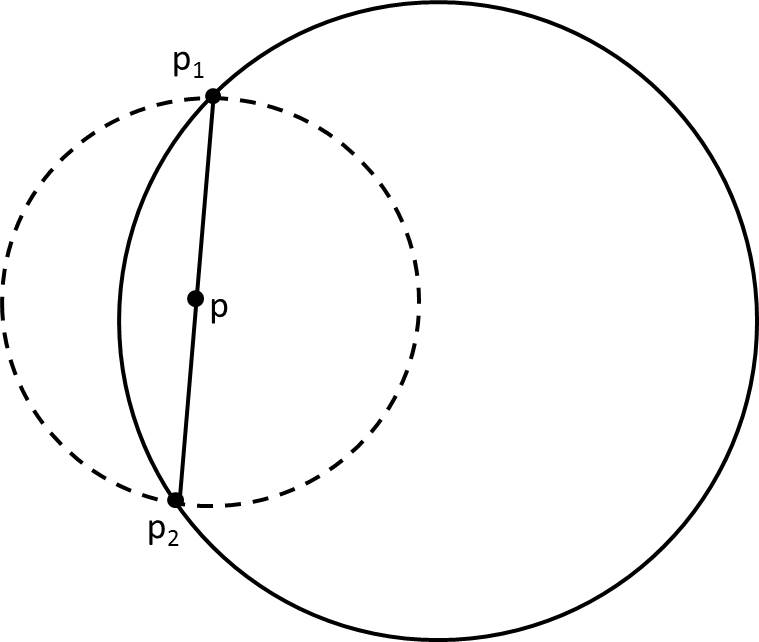
\includegraphics[scale=0.5]{images/cyclic-polygon.jpg}
\label{fig:cyclic-polygon}
\end{figure}

\begin{enumerate}
\item If $N(p) = \{p_1,p_2\}$, then no point in $P$ can lie on the arc joining $p_1$ and $p_2$ that is opposite to the center of the circle. Hence, $p_1$ and $p_2$ must be adjacent in the $k$-gon.  
\item If $N(p) \neq \{p_1,p_2\}$, then there are two possibilities.
\begin{enumerate}
\item Either $p_1$ and $p_2$ are not adjacent in the $k$-gon, or
\item The line joining $p_1$ and $p_2$ either passes through the center of the circle, or separates the rest of the polygon from the center of the circle. 
\end{enumerate}
In both cases, there can be at most one such pair $(p_1,p_2)$ in the polygon.
\end{enumerate}

Hence, we see that there would either be exactly $k-1$ or $k$ pairs $(p_1,p_2)$ such that $N(p) = \{p_1,p_2\}$, where $p$ is the midpoint of $p_1$ and $p_2$, and all such pairs are adjacent in the $k$-gon. Thus, they completely specify the order of the points in the $k$-gon.\footnote{In case of $k-1$ adjacent pairs, there is only one possibility left for the remaining edge.} 

Further, note that whether $N(p)$ is exactly the output of the voting rule $r$ on profile that consists of one occurrence of $p_1$ and one occurrence of $p_2$. Thus, it must be the same in both $f$ and $f'$. Hence, the order of points of $P$ in both $f$ and $f'$ must be identical, up to mirror image. Without loss of generality, assume that the order of the vertices is the same. If it is not, we take reflection, which does not change edge-lengths. 

Let the vertices be $\sigma_1, \sigma_2, \ldots, \sigma_k$ in order. We show that
\begin{equation}
\frac{\|\phi(\sigma_1)-\phi(\sigma_2)\|}{\|\phi'(\sigma_1)-\phi'(\sigma_2)\|} = \frac{\|\phi(\sigma_2)-\phi(\sigma_3)\|}{\|\phi'(\sigma_2)-\phi'(\sigma_3)\|} = \ldots = \frac{\|\phi(\sigma_k)-\phi(\sigma_1)\|}{\|\phi'(\sigma_k)-\phi'(\sigma_1)\|}
\label{eqn:polygon-condn}
\end{equation}

Take the triangle $\sigma_1, \sigma_2, \sigma_3$. In both $\phi$ and $\phi'$, the barycentric coordinates (linear combination of the vertices) of the circumcenter of the triangle must be equal, since the profile described by the barycentric coordinates must have output $\{\sigma_1,\ldots,\sigma_k\}$, which is only possible at the circumcenter of the $k$-gon. However, for triangle of side lengths $a$, $b$, and $c$, the barycentric coordinates are proportional to 
$$
(a^2 (b^2+c^2-a^2), b^2 (c^2+a^2-b^2), c^2 (a^2+b^2-c^2)).
$$
It can be easily shown that two triangles with identical barycentric coordinates of the circumcenter must have proportional side-lengths. Hence, we get 
$$
\frac{\|\phi(\sigma_1)-\phi(\sigma_2)\|}{\|\phi'(\sigma_1)-\phi'(\sigma_2)\|} = \frac{\|\phi(\sigma_2)-\phi(\sigma_3)\|}{\|\phi'(\sigma_2)-\phi'(\sigma_3)\|}
$$

Applying this repeatedly to triangles formed by all triplets of consecutive vertices gives \Cref{eqn:polygon-condn}. Finally, note that all the two-dimensional facets of the Delaunay triangulations $D_{\phi}$ and $D_{\phi'}$ are connected via shared edges. Thus, joining the \Cref{eqn:polygon-condn} of all polygons via shared edges, we get that for some $\lambda > 0$,
$$
\|\phi(\sigma)-\phi(\sigma')\| = \lambda \cdot \|\phi'(\sigma)-\phi'(\sigma')\|,
$$
for all $\sigma, \sigma'$, which is the final condition required.
\end{proof}
%%%%%%%%%%%%%%%%%%%%%%%%%%%%%%%%%%%%%%%%%%%%%
%%%%%%%%%%%%%%%%%%%%%%%%%%%%%%%%%%%%%%%%%%%%%
%%%%%%%%%%%%%%%%%%%%%%%%%%%%%%%%%%%%%%%%%%%%%

\section{Main Research Questions}
\begin{enumerate}
\item Proving that if $d$ is the minimum dimension required, then there exists a $d$-dimensional embedding.
\item Proving a generalization of the fact that all embeddings of a neutral SMPR are equivalent up to some sort of transformations and dimension uplifting. 
\item How to find the minimum dimension required for any given voting rule. What is the minimum dimension for PSR and the Kemeny rule?
\item Exploring MLE connection - efficient sampling.
\item Conditions imposed on the embeddings by other properties like monotonicity.
\end{enumerate}

\section{Other Research Questions}
\begin{enumerate}
\item Alternative proof of the characterization of positional scoring rules by observing that they are obtained by the same representation $R$ where $R_{\tau}$ is the permutation matrix generated by $\tau$ (which permutes rankings according to the mapping $\sigma \rightarrow \tau \sigma$), and different initial embeddings. 
\item Conjecture by Conitzer et al.~\cite{CRX09}: Consistent $+$ continuous $+$ neutral $\Leftrightarrow$ Neutral SRSF.
\item What about notions of consensus in Euclidean spaces other than mean $\rightarrow$ e.g., minimize maximum distance (everyone ``lets go'' equally)?
\end{enumerate}

\section{Scribbled Notes}
These are just high level intuitions. Need further investigations.
\begin{enumerate}
\item Neutral $\Rightarrow$ all rows permutations of each other $\Rightarrow$ sum = constant $\Leftrightarrow$ $[1,\ldots,1]$ is an eigenvector $\Leftrightarrow$ first coordinate of the embedding constant $\Leftrightarrow$ there is an embedding of rank-1

\item What is the permutation of all rankings generated by applying $\tau$ to each of them? What are all these $m!$ permutations?

\item Anything interesting about inner product maximizing rules that do not have embeddings of equal norm? Even symmetric ones may not be unanimous. 

\item An illustration: the \emph{Least Frequent Ranking Rule} is not SMPR - satisfies consistency, anonymity and neutrality. But violates unanimity. 
\end{enumerate}


%%%%%%%%%%%%%%%%%%%%%%%%%%%%%%%%%%%%%%%%%%%%%
%%%%%%%%%%%%%%%%%%%%%%%%%%%%%%%%%%%%%%%%%%%%%
%%%%%%%%%%%%%%%%%%%%%%%%%%%%%%%%%%%%%%%%%%%%%

\begin{comment}
Mean proximity rule / generalized scoring rule / SRSF - Neutral $\Rightarrow$ SRSF iff MLE
{\bf Question:} (Linear) Mean Proximity Rules - Captures all ``pairwise comparison scoring rules''?
\end{comment}

%%%%%%%%%%%%%%%%%%%%%%%%%%%%%%%%%%%%%%%%%%%%%
%%%%%%%%%%%%%%%%%%%%%%%%%%%%%%%%%%%%%%%%%%%%%
%%%%%%%%%%%%%%%%%%%%%%%%%%%%%%%%%%%%%%%%%%%%%

\bibliographystyle{plain}
\bibliography{abbshort,ultimate}
\end{document}